%%%%%%%%%%%%%%%%%%%%%%%%%%%%%%%%%%%%%%%%%
% Masters/Doctoral Thesis 
% LaTeX Template
% Version 2.1 (2/9/15)
%
% This template has been downloaded from:
% http://www.LaTeXTemplates.com
%
% Version 2.0 major modifications by:
% Vel (vel@latextemplates.com)
%
% Original authors:
% Steven Gunn  (http://users.ecs.soton.ac.uk/srg/softwaretools/document/templates/)
% Sunil Patel (http://www.sunilpatel.co.uk/thesis-template/)
%
% License:
% CC BY-NC-SA 3.0 (http://creativecommons.org/licenses/by-nc-sa/3.0/)
%
%%%%%%%%%%%%%%%%%%%%%%%%%%%%%%%%%%%%%%%%%

%----------------------------------------------------------------------------------------
%	PACKAGES AND OTHER DOCUMENT CONFIGURATIONS
%----------------------------------------------------------------------------------------

\documentclass[
11pt, % The default document font size, options: 10pt, 11pt, 12pt
%oneside, % Two side (alternating margins) for binding by default, uncomment to switch to one side
english, % ngerman for German
singlespacing, % Single line spacing, alternatives: onehalfspacing or doublespacing
%draft, % Uncomment to enable draft mode (no pictures, no links, overfull hboxes indicated)
%nolistspacing, % If the document is onehalfspacing or doublespacing, uncomment this to set spacing in lists to single
%liststotoc, % Uncomment to add the list of figures/tables/etc to the table of contents
%toctotoc, % Uncomment to add the main table of contents to the table of contents
%parskip, % Uncomment to add space between paragraphs
]{MastersDoctoralThesis} % The class file specifying the document structure

\usepackage[utf8]{inputenc} % Required for inputting international characters
\usepackage[T1]{fontenc} % Output font encoding for international characters

%\usepackage{palatino} % Use the Palatino font by default
\linespread{1.2}
\usepackage[margin = 1.25 in]{geometry}
\usepackage{wrapfig}
\usepackage{amsfonts}
\usepackage[utf8]{inputenc}
\usepackage[T1]{fontenc}
\usepackage{graphicx}
\usepackage[english]{babel}
\usepackage[algoruled]{algorithm2e}

\renewcommand{\theequation}{\thesection.arabic{equation}}

\renewcommand{\thefigure}{\thesection.\arabic{figure}}



\renewcommand{\vec}[1]{\mathbf{#1}}
\renewcommand{\theequation}{\thesubsection.\arabic{equation}}
\DeclareGraphicsExtensions{.pdf,.png,.jpg, .gif}

\usepackage{amsthm}

\usepackage[english]{babel}
\usepackage{mathtools}

%\usepackage[OT2,T1]{fontenc}
%\DeclareSymbolFont{cyrletters}{OT2}{wncyr}{m}{n}
%\DeclareMathSymbol{\sha}{\mathalpha}{cyrletters}{"58}

\DeclareFontFamily{U}{wncy}{}
\DeclareFontShape{U}{wncy}{m}{n}{<->wncyr10}{}
\DeclareSymbolFont{mcy}{U}{wncy}{m}{n}
\DeclareMathSymbol{\Sh}{\mathord}{mcy}{"58} 
\DeclareMathOperator*{\argmin}{arg\,min}

\newcounter{eqn}
\renewcommand*{\theeqn}{\alph{eqn})}
\newcommand{\num}{\refstepcounter{eqn}\text{\theeqn}\;}

\makeatother
\newcommand{\vectornorm}[1]{\left|\left|#1\right|\right|}
\newcommand*\conjugate[1]{\bar{#1}}

\newtheorem{thm}{Theorem}
\newtheorem{defn}{Definition}
 %\theoremstyle{plain}
  \newtheorem{theorem}{Theorem}[section]
  \newtheorem{corollary}[theorem]{Corollary}
  \newtheorem{proposition}[theorem]{Proposition}
  \newtheorem{lemma}[theorem]{Lemma}
\newtheorem{example}[theorem]{Example}
  \newtheorem{definition}[theorem]{Definition}
  \newtheorem{conj}[theorem]{Conjecture}
 \newtheorem{condition}{Condition}
 \newtheorem{remark}[theorem]{Remark}

\newcommand{\supp}{\operatorname{supp}} 
\newcommand{\vc}[1]{{\mathbf{ #1}}}
\newcommand{\tn}{\widetilde{\nabla}_{n} }
\newcommand{\Z}{{\mathbb{Z}}}
\newcommand{\re}{{\mathbb{R}}}
\newcommand{\II}{{\mathbb{I}}}
\newcommand{\ep}{{\mathbb{E}}}
\newcommand{\pr}{{\mathbb{P}}}
\newcommand{\FF}{{\mathcal{F}}}
\newcommand{\TT}{{\mathcal{T}}}
\newcommand{\phin}{\phig{n}}
\newcommand{\phig}[1]{\phi^{(#1)}}
\newcommand{\ol}[1]{\overline{#1}}
\newcommand{\eff}{{\rm eff}}
\newcommand{\suc}{{\rm suc}}
\newcommand{\tends}{\rightarrow \infty}
\newcommand{\setS}{{\mathcal{S}}}
\newcommand{\setP}{{\mathcal{P}}}
\newcommand{\setX}{{\mathcal{X}}}
\newcommand{\nec}{{\rm nec}}
\newcommand{\bd}{{\rm bd}}
%\usepackage[backend=bibtex,style=authoryear,natbib=true]{biblatex} % User the bibtex backend with the authoryear citation style (which resembles APA)

%\addbibresource{example.bib} % The filename of the bibliography

\usepackage[autostyle=true]{csquotes} % Required to generate language-dependent quotes in the bibliography

%----------------------------------------------------------------------------------------
%	THESIS INFORMATION
%----------------------------------------------------------------------------------------

\thesistitle{Compressive Wideband Spectrum Sensing for Cognitive Radios} % Your thesis title, this is used in the title and abstract, print it elsewhere with \ttitle
\supervisor{Dr Oliver Johnson, \\Dr Robert Pietchocki} % Your supervisor's name, this is used in the title page, print it elsewhere with \supname
\examiner{} % Your examiner's name, this is not currently used anywhere in the template, print it elsewhere with \examname
\degree{Doctor of Philosophy} % Your degree name, this is used in the title page and abstract, print it elsewhere with \degreename
\author{Thomas Kealy} % Your name, this is used in the title page and abstract, print it elsewhere with \authorname
\addresses{} % Your address, this is not currently used anywhere in the template, print it elsewhere with \addressname

\subject{Communications} % Your subject area, this is not currently used anywhere in the template, print it elsewhere with \subjectname
\keywords{} % Keywords for your thesis, this is not currently used anywhere in the template, print it elsewhere with \keywordnames
\university{\href{http://www.bris.ac.uk}{University of Bristol}} % Your university's name and URL, this is used in the title page and abstract, print it elsewhere with \univname
\department{\href{http://department.university.com}{Communications CDT}} % Your department's name and URL, this is used in the title page and abstract, print it elsewhere with \deptname
\group{\href{http://researchgroup.university.com}{Communications, Statistics}} % Your research group's name and URL, this is used in the title page, print it elsewhere with \groupname
\faculty{\href{http://faculty.university.com}{Faculty Name}} % Your faculty's name and URL, this is used in the title page and abstract, print it elsewhere with \facname

\hypersetup{pdftitle=\ttitle} % Set the PDF's title to your title
\hypersetup{pdfauthor=\authorname} % Set the PDF's author to your name
\hypersetup{pdfkeywords=\keywordnames} % Set the PDF's keywords to your keywords

\begin{document}

\frontmatter % Use roman page numbering style (i, ii, iii, iv...) for the pre-content pages

\pagestyle{plain} % Default to the plain heading style until the thesis style is called for the body content

%----------------------------------------------------------------------------------------
%	TITLE PAGE
%----------------------------------------------------------------------------------------

\begin{titlepage}
\begin{center}

\textsc{\LARGE \univname}\\[1.5cm] % University name
\textsc{\Large Doctoral Thesis}\\[0.5cm] % Thesis type

\HRule \\[0.4cm] % Horizontal line
{\huge \bfseries \ttitle}\\[0.4cm] % Thesis title
\HRule \\[1.5cm] % Horizontal line
 
\begin{minipage}{0.4\textwidth}
\begin{flushleft} \large
\emph{Author:}\\
\href{http://www.johnsmith.com}{\authorname} % Author name - remove the \href bracket to remove the link
\end{flushleft}
\end{minipage}
\begin{minipage}{0.4\textwidth}
\begin{flushright} \large
\emph{Supervisor:} \\
\href{http://www.jamessmith.com}{\supname} % Supervisor name - remove the \href bracket to remove the link  
\end{flushright}
\end{minipage}\\[3cm]
 
\large \textit{A thesis submitted in fulfilment of the requirements\\ for the degree of \degreename}\\[0.3cm] % University requirement text
\textit{in the}\\[0.4cm]
\groupname\\\deptname\\[2cm] % Research group name and department name
 
{\large \today}\\[4cm] % Date
%\includegraphics{Logo} % University/department logo - uncomment to place it
 
\vfill
\end{center}
\end{titlepage}

%----------------------------------------------------------------------------------------
%	DECLARATION PAGE
%----------------------------------------------------------------------------------------

\begin{declaration}
\addchaptertocentry{\authorshipname}

\noindent I, \authorname, declare that this thesis titled, \enquote{\ttitle} and the work presented in it are my own. I confirm that:

\begin{itemize} 
\item This work was done wholly or mainly while in candidature for a research degree at this University.
\item Where any part of this thesis has previously been submitted for a degree or any other qualification at this University or any other institution, this has been clearly stated.
\item Where I have consulted the published work of others, this is always clearly attributed.
\item Where I have quoted from the work of others, the source is always given. With the exception of such quotations, this thesis is entirely my own work.
\item I have acknowledged all main sources of help.
\item Where the thesis is based on work done by myself jointly with others, I have made clear exactly what was done by others and what I have contributed myself.\\
\end{itemize}
 
\noindent Signed:\\
\rule[0.5em]{25em}{0.5pt} % This prints a line for the signature
 
\noindent Date:\\
\rule[0.5em]{25em}{0.5pt} % This prints a line to write the date
\end{declaration}

\cleardoublepage

%----------------------------------------------------------------------------------------
%	QUOTATION PAGE
%----------------------------------------------------------------------------------------

\vspace*{0.2\textheight}

\noindent\enquote{\itshape Thanks to my solid academic training, today I can write hundreds of words on virtually any topic without possessing a shred of information, which is how I got a good job in journalism.}\bigbreak

\hfill Dave Barry

%----------------------------------------------------------------------------------------
%	ABSTRACT PAGE
%----------------------------------------------------------------------------------------

\begin{abstract}
\addchaptertocentry{\abstractname} % Add the abstract to the table of contents

The Thesis Abstract is written here (and usually kept to just this page). The page is kept centered vertically so can expand into the blank space above the title too\ldots

\end{abstract}

%----------------------------------------------------------------------------------------
%	ACKNOWLEDGEMENTS
%----------------------------------------------------------------------------------------

\begin{acknowledgements}
\addchaptertocentry{\acknowledgementname} % Add the acknowledgements to the table of contents

The acknowledgements and the people to thank go here, don't forget to include your project advisor\ldots

\end{acknowledgements}

%----------------------------------------------------------------------------------------
%	LIST OF CONTENTS/FIGURES/TABLES PAGES
%----------------------------------------------------------------------------------------

\tableofcontents % Prints the main table of contents

\listoffigures % Prints the list of figures

\listoftables % Prints the list of tables

%----------------------------------------------------------------------------------------
%	ABBREVIATIONS
%----------------------------------------------------------------------------------------

\begin{abbreviations}{ll} % Include a list of abbreviations (a table of two columns)

\textbf{LAH} & \textbf{L}ist \textbf{A}bbreviations \textbf{H}ere\\
\textbf{WSF} & \textbf{W}hat (it) \textbf{S}tands \textbf{F}or\\

\end{abbreviations}

%----------------------------------------------------------------------------------------
%	PHYSICAL CONSTANTS/OTHER DEFINITIONS
%----------------------------------------------------------------------------------------

%\begin{constants}{lr@{${}={}$}l} % The list of physical constants is a three column table

% The \SI{}{} command is provided by the siunitx package, see its documentation for instructions on how to use it

%Speed of Light & $c$ & \SI{2.99792458e8}{\meter\per\second} (exact)\\
%Constant Name & $Symbol$ & $Constant Value$ with units\\

%\end{constants}

%----------------------------------------------------------------------------------------
%	SYMBOLS
%----------------------------------------------------------------------------------------

%\begin{symbols}{lll} % Include a list of Symbols (a three column table)

%$a$ & distance & \si{\meter} \\
%$P$ & power & \si{\watt} (\si{\joule\per\second}) \\
%Symbol & Name & Unit \\

%\addlinespace % Gap to separate the Roman symbols from the Greek

%$\omega$ & angular frequency & \si{\radian} \\

%\end{symbols}

%----------------------------------------------------------------------------------------
%	DEDICATION
%----------------------------------------------------------------------------------------

\dedicatory{For/Dedicated to/To my\ldots} 

%----------------------------------------------------------------------------------------
%	THESIS CONTENT - CHAPTERS
%----------------------------------------------------------------------------------------

\mainmatter % Begin numeric (1,2,3...) page numbering

\pagestyle{thesis} % Return the page headers back to the "thesis" style

% Include the chapters of the thesis as separate files from the Chapters folder
% Uncomment the lines as you write the chapters

\chapter{The Probabilistic group testing problem}
Group testing is a sparse inference problem, first introduced by Dorfman \cite{dorfman} in the context of testing for rare diseases.
Given  a large population of items $\setP$,
indexed by \( \{1, \ldots N\}\), where
some small fraction of the items are interesting in some way, how can we find the interesting items efficiently? 

We perform a sequence of $T$ pooled tests defined by test sets $\setX_1, \ldots, \setX_T$, where each $\setX_i \subseteq \setP$. 
We represent the interesting (`defective') items by 
a random vector $\vc{U} = ( U_1, \ldots, U_N)$, where $U_i$ is the indicator of the event that item $i$ is defective. 
For each test $i$, we jointly 
test all the items in $\setX_i$, and the outcome $y_i$ is `positive' ($y_i = 1$) if and only if any item in $\setX_i$ is defective. In other words, 
$y_i = \II \left( \sum_{j \in \setX_i} U_j \geq 1\right)$, since for simplicity we are  considering the noiseless case. Further, in this paper, we restrict our attention to
 the adaptive case, where we choose test set
$\setX_i$ based on a knowledge of sets $\setX_1, \ldots, \setX_{i-1}$ and outcomes $y_1, \ldots, y_{i-1}$. The group testing problem requires us to infer $\vc{U}$ with high
probability given a low number of tests $T$.

Since Dorfman's paper \cite{dorfman}, there has been considerable work on the question of how to design the sets $\setX_i$ in order to minimise the number of tests $T$
required. In this context, we briefly mention so-called combinatorial designs (see \cite{du, malyutov} for a summary, with \cite{malyutov} giving invaluable
references to an extensive body of Russian work in the 1970s and 1980s). Such designs typically aim to ensure that 
set-theoretic properties known as disjunctness
and separability occur. In contrast, for simplicity of analysis, as well as  performance of optimal order, it is possible to consider random designs. Here sets $\setX_i$ are chosen
at random, either using constructions such as independent Bernoulli designs \cite{atia, johnsonc8, johnson33} or more sophisticated  random designs based on LDPC codes \cite{wadayama}. 

Much previous work has focussed on the Combinatorial group testing problem, where there are a fixed number of defectives $K$, and the defectivity vector $\vc{U}$ is chosen uniformly among all
binary vectors of weight $K$. In contrast, in this paper we study a Probabilistic group testing problem as formulated
for example in the work of Li et al. \cite{li5}, in that we suppose 
 each item is defective  independently with probability \(p_i\), or equivalently take $U_i$ to be independent Bernoulli($p_i$).

This Probabilistic framework, including non-uniform priors, is natural for many applications of group testing.
For example, see \cite{atia2}, the cognitive radio problem can be formulated in terms of  a population
 of communication bands in frequency spectra with some (unknown) occupied bands you must not utilise. Here, the values of $p_i$ may be chosen
 based on some database of past spectrum measurements or other prior information. Similarly, as in Dorfman's original work  \cite{dorfman} or more recent 
research \cite{shental} involving screening for genetic conditions, values of
$p_i$ might summarise prior information based on a risk profile or  family history.
%
\subsection{Group testing capacity}
%
It is possible to characterize performance tradeoffs in group testing 
 from an information-theoretic point of view -- see for example \cite{atia, johnsonc10, johnson33, tan}. These papers have focussed on group testing as a channel coding problem, 
with \cite{atia, tan}
explicitly calculating the mutual information.
The paper \cite{johnsonc10} defined the capacity of a Combinatorial group testing procedure, which characterizes the number of bits of information
about the defective set which we can learn per test. We give a more general definition here,
which covers both the Combinatorial and Probabilistic cases.
%
\begin{definition} \label{def:capacity} Consider a sequence of group testing problems where the $i$th problem
has defectivity vector  $\vc{U}^{(i)}$, and consider algorithms which are given $T(i)$ tests.
We refer to a constant $C$ as the (weak) group testing capacity if for any $\epsilon > 0$:
  \begin{enumerate}
    \item any sequence of algorithms with
      \begin{equation} \label{eq:lower}
        \liminf_{i \tends} \frac{ H(\vc{U}^{(i)}) }{T(i)} \geq C+ \epsilon,
      \end{equation}
      has success probability $\pr(\suc)$ bounded away from 1,
    \item and there exists a sequence of algorithms with
      \begin{equation} \label{eq:upper}
        \liminf_{i \tends} \frac{H(\vc{U}^{(i)}) }{T(i)}  \geq C - \epsilon
      \end{equation}
      with success probability $\pr(\suc) \rightarrow 1$.
  \end{enumerate}
\end{definition}
%
\begin{remark}
In the Combinatorial case of $K$ defective items with all defective sets equally
likely, $ H(\vc{U}) = \log_2 \binom{N}{K}$, which is the term found in the denominator in \cite[Eq. (1) and (2)]{johnsonc10}. In the Probabilistic case (as in \cite{li5}) 
 we know $H(\vc{U}) = -\sum_{i=1}^N h(p_i)$ where $h(t) = -t \log_2 t - (1-t) \log_2(1-t)$ is the binary entropy function. 
\end{remark}
%
\begin{remark} If for $ \liminf_{i \tends} \frac{ H(\vc{U}^{(i)}) }{T(i)} \geq C+ \epsilon$, the success probability 
$\pr(\suc) \rightarrow 0$ we say that $C$ is the strong group testing capacity, following standard terminology in information
theory. Such a result is referred to as a strong converse.
\end{remark}

\subsection{Main results}

The principal contribution of \cite[Theorem 1.2]{johnsonc10} was the following result:
%
\begin{theorem}
[\cite{johnsonc10}] \label{thm:mainold}
The strong capacity of the adaptive noiseless Combinatorial group testing problem
  is  $C = 1$,
  in any regime such that $K/N \rightarrow 0$.
\end{theorem}
%
This argument came in two parts. First, in \cite[Theorem 3.1]{johnsonc10} the authors  proved a new
upper bound on success probability 
\begin{equation} \label{eq:bja} \pr(\suc) \leq \frac{2^T}{\binom{N}{K}}, \end{equation} which implied a strong converse ($C \leq 1$). This was complemented 
by 
showing that, in the Combinatorial case, an algorithm based on 
Hwang's Generalized Binary Splitting Algorithm (HGBSA) \cite{hwang}, \cite{du} is essentially optimal in the required sense,
showing that $C=1$ is achievable.


It may be useful to characterize the Probabilistic group testing problem in 
terms of the effective sparsity $\mu^{(N)}: = \sum_{i=1}^N p_i$. In particular, if the $p_i$ are (close to) identical, we would expect performance similar to that in the Combinatorial
case with $K = \mu^{(N)}$ defectives. As in \cite{johnsonc10}, we  focus on asymptotically sparse cases, where $\mu^{(N)}/N \rightarrow 0$. In contrast, Wadayama
\cite{wadayama} considered a model where $p_i$ are identical and fixed.
The main result of the present paper is Theorem \ref{thm:main}, stated and proved in Section \ref{sec:main} below, which implies the 
following  Probabilistic group testing version of Theorem \ref{thm:mainold}.
 %
\begin{corollary} \label{cor:main}
 In the case where $p_i \equiv p$, the weak capacity of the adaptive noiseless Probabilistic group testing problem
  is  $C = 1$, in any regime such that $\mu^{(N)}/N \rightarrow 0$ and $\mu^{(N)} \rightarrow \infty$.
  \end{corollary}



Again we prove our main result Theorem \ref{thm:main} using complementary bounds on both sides. First in Section \ref{sec:ub} we recall
 a universal upper bound on success probability, Theorem \ref{thm:upper}, taken from
\cite{li5}, which implies a weak converse.   In \cite{li5}, Li et al. introduce
the Laminar Algorithm for Probabilistic group testing.  
In Section \ref{sec:algo} we propose a refined version of this Laminar Algorithm, based on Hwang's HGBSA \cite{hwang}, which is
analysed in Section \ref{sec:main}, and shown to imply performance close to optimal in the sense of capacity.

Bounds of [\cite{li5}] (see Theorem \ref{thm:lower} below) which shows that \(10eH\left(\textbf{U}\right)\) tests are required to guarantee convergence to zero success probability. Our calculation is to improve this to \(H\left(\textbf{U}\right)\) plus an error term , which is optimal up to the size of the error term.

\section{Algorithms and existing results}

\subsection{Upper bounds on success probability} \label{sec:ub}

Firstly \cite[Theorem 1]{li5} can be restated to give the following
upper bound on success probability:
%
\begin{theorem} \label{thm:upper}
Any Probabilistic group testing algorithm using $T$ tests with noiseless measurements has success probability satisfying
$$ \pr(\suc) \leq \frac{T}{H( \vc{U})}.$$
\end{theorem}

Rephrased in terms of Definition \ref{def:capacity}, this tells us that the weak capacity of noiseless Probabilistic 
group testing is $\leq 1$. The logic is as follows; if the capacity were
$1 + 2 \epsilon$ for some $\epsilon > 0$, then there would exist a sequence of algorithms with $H(\vc{U}^{(i)})/T(i) \geq 1 + \epsilon$ with success probability tending to 1.
However, by Theorem \ref{thm:upper}, any such algorithms have $\pr(\suc) \leq 1/(1+\epsilon)$, meaning that we have 
established that a weak converse holds.

\begin{remark}
It remains an open and interesting problem to prove an equivalent of \eqref{eq:bja} as in \cite[Theorem 3.1]{johnsonc10}. That is we hope to find an upper bound
on success probability in a form  which implies a strong converse, and hence that the strong capacity of Probabilistic group
testing is equal to 1.
\end{remark}

\subsection{Binary search algorithms}

The main contribution of this work is  to describe and analyse algorithms that will find the defective items.
In brief, we can think of Hwang's HGBSA algorithm as dividing the population $\setP$ into search sets $\setS$. First, all the items in a search set $\setS$ are tested together,
using a test set $\setX_1 = \setS$. If the result is negative
($y_1 = 0$), we can be certain that $\setS$ contains no defectives. However, if the result is positive ($y_1 = 1$),  $\setS$ must contain at least one defective.

If $y_i = 1$, we can be guaranteed to find at least
one defective, using the following binary search strategy.  
We  split the   set $\setS$ in two, and test the `left-hand' set, say $\setX_{2}$. If $y_{2} = 1$, then we know that $\setX_{2}$ contains at least one defective.
If $y_{2} = 0$, then $\setX_{2}$ contains no defective, so we can deduce that $\setS \setminus \setX_2$ contains at least one defective. By repeated use of this strategy, we are 
guaranteed to find a succession of nested sets which contain at least one defective, until $\setX_i$ is of size 1, and we have isolated a single defective item.

However this strategy may not find every defective item in $\setS$. To be specific, it is possible that at some stage
both the left-hand and right-hand sets contain a defective. The Laminar Algorithm of \cite{li5} essentially deals with this by testing 
both sets. However, we believe that this is inefficient, since typically both sets will not contain a defective. Nonetheless, the Laminar Algorithm satisfies
 the following  performance guarantees  proved in \cite[Theorem 2]{li5}: 
%
\begin{theorem} \label{thm:lower}
The expected number of tests required by the Laminar Algorithm \cite{li5}  is $\leq 2 H(\vc{U}) + 2 \mu$. Under a technical condition (referred to as non-skewedness), the
success probability can be bounded by $\pr(\suc) \geq 1- \epsilon$ using $T = (1+ \delta) (2^{\Gamma + \log_2 3} + 2) H(\vc{U})$ tests, where $\Gamma$ is defined implicitly
in terms of $\epsilon$, and $\delta \geq 2 e - 1$.
\end{theorem}

Ignoring the $\Gamma$ term, and assuming the non-skewedness condition holds,
 this implies that (using the methods of \cite{li5}) $T =  2 e (3 + 2) H(\vc{U}) = 10 e H(\vc{U})$ tests are required to guarantee convergence to $1$
of the success probability. In our language, this implies a lower bound of $C \geq 1/(10 e) = 0.0368$. Even ignoring the analysis of error probability, the fact that the expected number
of tests is $\leq 2 H(\vc{U}) + 2 \mu$ suggests that we cannot hope to achieve $C > 1/2$ using the Laminar Algorithm.
%
\subsection{Summary of our contribution} \label{sec:algo}

\begin{algorithm}
% \SetLine 
 %\SetAlgoLined % For previous releases [?]
 \KwData{A Set \(S\) of \(\lvert S \rvert = n\) items, \(\mu\) of which are actually defective in expectation, a probability vector \( \vec{p}^{\left(n\right)} \) describing each item's independent probability of being defective, and a cutoff \(\theta\)}
 \KwResult{The set of defective items}
 Discard items with \(p_i \leq \theta\)
 \\
 Sort the remaining items into \(B\) bins, collecting items together with \(p_i \in \left[1/2C^r,1/2C^{r-1}\right)\) in bin \(r\).
 \\
 Sort the items in each bin into sets s.t. the (normalised) probability of each set is less than \(1/2\).
 \\
 Test each set in turn
 \\
   	\If{The test is positive}{Arrange the items in the set on a Shannon-Fano/Huffman Tree and search the set for all the defectives it contains}

 \caption{Algorithm for the non-iid group testing problem}
\end{algorithm}

The main contribution of our paper is a refined version of the Laminar Algorithm, summarised above, and an analysis resulting in tighter error bounds as formulated in Proposition \ref{prop:overall} (in terms of expected number of tests) and Theorem \ref{thm:main} (in terms
of error probabilities).
The  key ideas are:
\begin{enumerate}
\item To partition the population $\setP$ into search  sets  $\setS$ containing items which have similar probabilities,
expressed through the Bounded Ratio Condition \ref{cond:ratio}. This is discussed in Section \ref{sec:boundedratio}, and optimised in the proof
of Proposition \ref{prop:overall}.
\item The way in which we deal with sets $\setS$ which contain more than one defective, as discussed in Remark \ref{rem:algo} below. Essentially we do not backtrack after each test by
testing both left- and right-hand sets, but only backtrack after each defective is found.
\item To discard items which have probability below a certain
threshold, since with high probability none of them will be defective. This is an idea introduced in \cite{li5} and discussed
in Section \ref{sec:discard}, with a new bound given in Lemma \ref{lem:thresh}.
\item  Careful analysis in Section \ref{sec:expectation} of the properties of search sets $\setS$ gives Proposition \ref{prop:overall}, which shows that the expected number of tests required can
be expressed as $H(\vc{U})$ plus an error term. In Section \ref{sec:main},
we give an analysis of the error probability using Bernstein's inequality, Theorem \ref{thm:bernstein}, allowing us to
prove Theorem \ref{thm:main}.
\end{enumerate}
%


\subsection{Wider context: sparse inference problems}

Recent work \cite{aksoylar,tan} has shown that many arguments and bounds hold in a common framework of sparse inference
which includes group testing and compressive sensing.

Digital communications, audio, images, and text are examples of data sources we can compress. We can do this, because these data sources are sparse: they have fewer degrees of freedom than the space they are defined upon. 
For example, images have a well known expansion in either the Fourier or Wavelet bases. The text of an English document will only be comprised of words from the English dictionary, and not all the possible strings from the space of strings made up from the characters \(\{a, \ldots, z \}\). 

Often, once a signal has been acquired it will be compressed. However, the compressive sensing paradigm introduced by
\cite{candes,donoho2} shows that this isn't necessary. In those papers it was shown that a 'compressed' representation of a signal could be obtained from random linear projections of the signal and some other basis (for example White Gaussian Noise). The question remains, given this representation how do we recover the original signal? For real signals, a simple linear programme suffices.
Much of the work in this area has been couched in terms of the sparsity of the signal and the various bases the signal can be represented in (see for example \cite{candes,donoho2}). 


\section{Analysis and new bounds}

\subsection{Searching a set of bounded ratio} \label{sec:boundedratio}

Recall that we have a population $\setP$ of items to test, each with associated probability of defectiveness $p_i$.
The strategy of the proof is to partition $\setP$ 
 into search sets $\setS_1, \ldots, \setS_G$, each of which contains items which have
comparable values of $p_i$.

\begin{condition}[Bounded Ratio Condition] \label{cond:ratio}
Given $C \geq 1$, say that a set $\setS$ satisfies the Bounded Ratio Condition with constant $C$ if
\begin{equation} \label{eq:ratio} \max_{i,j \in \setS} \frac{p_j}{p_i} \leq C.\end{equation} \end{condition}
%
(For example clearly if $p_i \equiv p$, any set $\setS$ satisfies the condition for any $C \geq 1$).
%
\begin{lemma} \label{lem:sfstep}
Consider a set $\setS$ satisfying the Bounded Ratio Condition  with constant $C$
and write $P_{\setS} = \sum_{j \in \setS} p_j$.
In a  Shannon--Fano tree for the probability distribution $\ol{p}_i := p_i/P_{\setS}$, each item has length $\ell_i^{(\setS)}$
bounded by
\begin{equation} \label{eq:depth} \ell_i^{(\setS)} \leq \ell_{\max}^{(\setS)} := \frac{h(\setS)}{P_{\setS}} + \log_2  C + \log_2  P_{\setS} + 1,\end{equation}
where we write $h( \setS) :=  -\sum_{j \in \setS} p_j \log_2  p_j$.
\end{lemma}
\begin{proof} Under the Bounded Ratio Condition, for any $i$ and $j$, we know that by taking logs of \eqref{eq:ratio}
$$ -\log_2 p_i \leq - \log_2 p_j + \log_2 C.$$
Multiplying by $p_j$ and summing over all $j \in \setS$, we obtain that
\begin{equation} \label{eq:setbd} -P_{\setS} \log_2 p_i \leq h(\setS) + P_{\setS} \log_2 C.\end{equation}
Now, the Shannon--Fano length of the $i$th item is

\begin{eqnarray}
 \ell_i^{(\setS)} &= \lceil -\log_2 \ol{p}_i \rceil \\
&\leq &  -\log_2 p_i + \log_2 P_{\setS} + 1 \label{eq:lengthbd} \\
& \leq  & \left(\frac{h(\setS)}{P_{\setS}} + \log_2 C \right) + \log_2 P_{\setS} + 1. \nonumber
\end{eqnarray}

and the result follows by \eqref{eq:setbd}.
\end{proof}

Next we describe our search strategy:

\begin{remark} \label{rem:algo}
Our version of the algorithm will find every defective in a set $\setS$. We start as before by testing every item in $\setS$ together. If this test is negative, we are done.
Otherwise, if it is positive, we can perform binary search as section II-B to find one defective item, say $d_1$. Now, test every item in $\setS \setminus \{ d_1 \}$ together.
If this test is negative, we are done, otherwise we repeat the search step on this smaller set, to find another defective item
$d_2$, then we test $\setS \setminus \{ d_1, d_2 \}$ and so on.

We think of the algorithm as repeatedly searching a binary tree. Clearly, if the tree has depth bounded by $\ell$, then the search will take $ \leq \ell$ tests to find one defective. In total, 
if the set contains $U$ defectives, we need to repeat $U$ rounds of searching, plus the final test to guarantee that the set contains no more defectives, so will use $\leq \ell U + 1$ tests.
\end{remark}

\begin{lemma} \label{lem:expset}
 Consider a search set $\setS$ satisfying the Bounded Ratio Condition  and write $P_{\setS} = \sum_{j \in \setS} p_j$.
If (independently) item $i$ is defective with probability $p_i$, 
we can recover  all defective items in the set using $T_\setS$ tests, where $\ep T_\setS \leq T_{\bd}(\setS)$ for
\begin{equation} \label{eq:tbds}
 T_{\bd}(\setS) :=  h(\setS) +  P_{\setS} \log_2 C +  P_{\setS} \log_2 P_{\setS} + P_\setS + 1. \end{equation}
\end{lemma}
\begin{proof}
Using the algorithm of Remark \ref{rem:algo}, laid out on the Shannon-Fano tree constructed in Lemma \ref{lem:sfstep}, we are guaranteed  to find every defective.
The number of tests to find one defective thus corresponds to the depth of the tree, which is bounded by  $\ell_{\max}^{(\setS)}$ given in \eqref{eq:depth}.

Recall that we write $U_i$ for the indicator of the event that the $i$th item is defective, we will write $U_{\setS} = \sum_{i \in \setS} U_i$ for the total number of defectives in \(\setS\), and 
$l_i^{(\setS)}$ for the length of the word in the Shannon Fano tree. As discussed in Remark \ref{rem:algo}
this search procedure will take 
\begin{eqnarray}
T_\setS & = &  1 + \sum_{i \in \setS} U_i \ell_i^{(\setS)} \nonumber \\
& = &  \sum_{i \in \setS} p_i \ell_i^{(\setS)} + 1 + \sum_{i \in S} \ell_i^{(\setS)} (U_i - p_i)  \nonumber \\
& \leq & \sum_{i \in \setS} p_i \ell_{\max}^{(\setS)} +  1 + \sum_{i \in \setS} V_i^{(\setS)}  \nonumber \\
& =  &  P_{\setS} \ell_{\max}^{(\setS)} +  1 + \sum_{i \in S} V_i^{(\setS)} \nonumber \\
& \leq  & T_{\bd}(\setS) + \sum_{i \in S} V_i^{(\setS)} 
\mbox{ \;\; tests.} \label{eq:testsperdef} \end{eqnarray}
Here we write $V_ i^{(\setS)} = \ell_i^{(\setS)} (U_i - p_i)$, which has expectation zero, and \eqref{eq:testsperdef} follows using the expression for 
$\ell_{\max}^{(\setS)}$ given in   Lemma \ref{lem:sfstep}.
\end{proof}

\subsection{Discarding low probability items} \label{sec:discard}

As in \cite{li5}, we use a probability threshold $\theta$, and write $\setP^*$ for the population having removed items with $p_i \leq \theta$.
If an item lies in $\setP \setminus \setP^*$ we do not 
test it, and simply mark it as non-defective. This truncation operation gives an error if and only if some item in $\setP \setminus \setP^*$ is defective.
By the union bound, 
this truncation operation contributes a total of $\pr( \mbox{$\setP \setminus \setP^*$ contains a defective}) \leq  \rho := \sum_{i=1}^n p_i \II(p_i \leq \theta)$ to the error probability.



\begin{lemma} \label{lem:thresh}
Choosing $\theta(P_e)$ such that  
\begin{equation} \label{eq:thetadef}
-\log_2 \theta(P_e) = \min\left( \log_2  \left( \frac{2n}{P_e} \right), \frac{2 H( \vc{U})}{P_e} \right)
\end{equation}
ensures that  
\begin{equation}
\pr(\mbox{ $\setP \setminus \setP^*$ contains a defective} ) \leq P_e/2. \label{eq:setpstar} \end{equation} \end{lemma}
\begin{proof}
The approach of \cite{li5} is essentially to bound $\II(p_i \leq \theta) \leq \theta/p_i$ so that
$\rho = \sum_{i=1}^n p_i \II(p_i \leq \theta) \leq \sum_{i=1}^n p_i (\theta/p_i) = n \theta$. Hence, choosing a threshold
of $\theta = P_e/(2n)$ guarantees the required bound on $\rho$.

We combine this with another bound, constructed using a different function:
 $\II(p_i \leq \theta) $ $\leq (-\log_2 p_i)/(-\log_2 \theta)$, so that
$$ \rho = \sum_{i=1}^n p_i \II(p_i \leq \theta) \leq \sum_{i=1}^n p_i  \left( 
\frac{-\log_2 p_i}{-\log_2 \theta } \right) \leq \frac{H( \vc{U})}{-\log_2 \theta},$$ 
so we deduce the result. \end{proof}

\subsection{Searching the entire set} 

Having discarded items with $p_i$ below
this probability threshold $\theta$ and given bounding ratio $C$,
we create a series of bins. We collect together items with probabilities $p \in [1/2,1]$ in bin 0,
$p \in [1/(2C), 1/2)$ in bin 1, items with probabilities $p \in [1/(2C^2), 1/(2C))$ in bin 2, \ldots, and items with probabilities $p \in 
[1/(2C^B), 1/(2C^{B-1}))$ in bin $B$.

The probability threshold $\theta$ means that
there will be a finite number of such bins, with the index $B$ of the last bin defined by the fact that $1/(2C^B) \leq
\theta < 1/(2C^{B-1})$, meaning that $(B -1) \log_2 C < - \log_2 (2 \theta)$, so
\begin{equation} \label{eq:bincount} B \leq  \frac{ - \log_2 (2 \theta)}{\log_2 C} + 1. \end{equation}

We split the items in each bin into search sets $\setS_i$, motivated by the following definition:

\begin{definition} \label{def:full}
A set of items \( \setS \) is said to be \(full\) if $P_{\setS} = \sum_{i \in \setS} p_i \geq \frac{1}{2}$.
\end{definition}

Our splitting procedure is as follows: we create a list of
possible sets $\setS_1, \setS_2, \ldots $. For $i$ increasing from $0$ to $B$,
we place items from bin $i$ into sets $\setS_{b_{i}+1}, \ldots, \setS_{b_{i+1}}$, for some $b_i$, where $b_{0} = 0$.
Taking the items 
from bin $i$, while $\setS_{b_{i}+1}$ is not full  (has 
total probability $< \frac{1}{2}$) we will place  items into it. Once enough items have been added to fill $\setS_{b_{i} + 1}$,
we will proceed in the same way to fill $\setS_{b_{i}+2}$, and so on until all the items in bin $i$ have been
assigned to sets $\setS_{b_{i}+1}, \ldots, \setS_{b_{i+1}}$,  where $\setS_{b_{i+1}}$ may remain not full.
%
\begin{proposition} \label{prop:splitting}
 This splitting procedure will divide $\setP^*$ into search sets $\setS_1, \ldots, \setS_G$, where
the total number of sets is 
$$ G \leq 2 \mu + B \leq 2 \mu  +  \left( \frac{ -\log_2 (2\theta)}{\log_2 C} + 1 \right).$$ 
Each set $\setS_j$ satisfies the Bounded Ratio Condition and has total probability $P_j := P_{\setS_j} \leq 1$. \end{proposition}
\begin{proof}
First, note that  
the items from bin $0$ each lie in a set $\setS$ on their own.
These sets will be full, trivially satisfy the Bounded Ratio Condition \ref{cond:ratio}
with constant $C$,
 and have probability satisfying $P_j \leq 1$.
 For each of bins $1, \ldots, B$:
\begin{enumerate}
\item  \label{it:count} For each bin $i$,
it is possible that the last set $\setS_{b_{i+1}}$  will not be full, but every other
set corresponding to that bin will be full. Hence, there are no more than $B$ sets which are not full.
\item For each resulting set $\setS_j$, the total probability $P_j \leq 1$ (since just before we add the final item, $\setS_j$ is not full, so at
that stage has total probability $\leq 1/2$, and each element in bins $1, \ldots, B$ has probability $\leq 1/2$).
\item Since each set $\setS_j$ contains items  taken from the same bin, it will satisfy the Bounded Ratio Condition  with 
constant $C$.
\end{enumerate}

 Note that the number of full sets is \(\leq 2 \mu \), since
\begin{align} 
\label{eq:counting}
\mu &=  \sum_{i \in \setP} p_i \\ 
&\geq \sum_{i \in \setP^*} p_i  = \sum_{j=1}^G P_j
\\ &\geq
\sum_ {\mbox{\scriptsize $j$: $\setS_j$ full}} P_j \geq \left| \mbox{$\setS_j$ full} \right| \frac{1}{2}. \end{align}
Since, as discussed  in point \ref{it:count}) above,
 the total number of sets is bounded by the number of full sets plus $B$, the result follows using Equation
(\ref{eq:bincount}).
\end{proof}

\subsection{Bounding the expected number of tests} \label{sec:expectation}
%
We allow the algorithm to work until all defectives in $\setP^*$ are found, and write $T$ for the (random) number of tests this takes.
%
\begin{proposition} \label{prop:overall} Given a population $\setP$
where (independently) item $i$ is defective with probability $p_i$,  
we  recover  all defective items in $\setP^*$ in $T$ tests with $\ep T \leq T_{\bd}$, where
\begin{equation} \label{eq:tbd}
 T_{\bd} := \left( H( \vc{U}) + 3 \mu + 1 \right) +  
 2 \sqrt{ \mu  \left( -\log_2 (2\theta) \right)}.
\end{equation}
\end{proposition}
\begin{proof} Given a value of $C$,
Proposition \ref{prop:splitting} shows that our splitting procedure divides $\setP^*$ into 
$G$ sets $\setS_1, \ldots, \setS_G$, such that each set $\setS_j$ satisfies the Bounded Ratio Condition with constant $C$ and has total probability $P_j
\leq 1$. Using the notation of Lemma \ref{lem:expset}, $T = \sum_{j=1}^G T_{\setS_j}$, where 
$\ep T_{\setS_j} \leq  T_{\bd}(\setS_j)$.

Adding this bound over the different sets, since $P_j \leq 1$ means that $P_j \log_2 P_j \leq 0$, we obtain
\begin{align} \label{eq:total}
\lefteqn{ \sum_{j=1}^G T_{\bd}(\setS_j) } \nonumber \\
&\leq \sum_{j=1}^G \left(  h(\setS_j)  + P_j (\log_2 C+1) + 1 \right) \nonumber \\
&= \sum_{j \in \setP^*} -p_j \log_2 p_j + \mu  (\log_2 C+1) + G \nonumber \\
&\leq \sum_{j \in \setP^*} h(p_j)  + 3 \mu  +  1 + \left( \frac{ -\log_2 (2\theta)}{\log_2 C} +  \mu  \log_2 C \right)  
\nonumber \\
&\leq \left( H( \vc{U}) + 3 \mu + 1 \right) \\ 
&+  \left( \frac{ -\log_2 (2 \theta)}{\log_2 C} +  \mu \log_2 C \right).
\label{eq:toopt}
\end{align}
This follows by the bound on $G$ in Proposition \ref{prop:splitting}, as well as 
the fact that $ 0 \leq p_j \leq 1$ means that 
 for any $i$, $ - p_j \log_2 p_j =  (1-p_j) \log_2 (1-p_j) + h(p_j) \leq h(p_j)$.

Finally, we  choose $C > 1$ to optimize the  second bracketed term in Equation (\ref{eq:toopt}).
Differentiation shows that the optimal $C$ satisfies $\log_2 C = \sqrt{ -\log_2 (2 \theta)/\mu},$ meaning that
 the 
bracketed term $$
\frac{ -\log_2 (2 \theta)}{\log_2 C} +  \mu \log_2 C  =
 2 \sqrt{ \mu  \left( -\log_2 (2\theta) \right)} ,$$
and the result follows.
\end{proof}

\subsection{Controlling the error probabilities} \label{sec:main}
%
Although Section \ref{sec:expectation} proves that $\ep T \leq T_{\bd}$,
 to bound the capacity, we need to prove that with high probability
$T$ is not significantly larger than $T_{\bd}$. This can be done using
 Bernstein's inequality (see for example Theorem 2.8 of \cite{petrov}):
%
\begin{theorem}[Bernstein] \label{thm:bernstein}
For zero-mean random variables $V_i$ which are uniformly bounded by $|V_i| \leq M$,
if we write $L  := \sum_{j=1}^n \ep V_j^2 $
 then
\begin{equation} \pr \left( \sum_{j=1}^n V_j \geq t \right)  \leq  \exp \left( - \frac{ t^2}{4 L}  \right),  \mbox{
for any $0 \leq t \leq \frac{L}{M}$.}   \label{eq:bernstein}
\end{equation}
\end{theorem}
%
We deduce the following result:
%
\begin{theorem} \label{thm:main}
Write  $L = \sum_{j \in \setP^*} l_j^2 p_j (1-p_j)$,  $M = -\log_2 \theta+1$
and $\psi = (L/(4M^2))^{-1/3}$.
Define
\begin{equation} \label{eq:tnec}
 T_{\nec} = T_{\bd} + \psi H(\vc{U}), \end{equation}
where $T_{\bd} $ is given in \eqref{eq:tbd}.
\begin{enumerate}
\item \label{it:part1} If we terminate our group testing algorithm after
$T_{\nec}$ tests, the success probability
\begin{equation} \label{eq:errorprob} 
\pr(\suc) \geq 1 - \frac{1}{2} \sqrt{ \frac{\mu}{H(\vc{U}) }} -  \exp \left( - \left( \frac{L}{4  M^2 }  \right)^{1/3}
\right).
\end{equation}
\item \label{it:part2}
Hence  in any regime where $\mu \rightarrow \infty$ with
 $\mu/H(\vc{U}) \rightarrow 0$ and $L/M^2 \rightarrow \infty$,  
our group testing algorithm has  (a) $ \liminf H(\vc{U})/T_{\nec} \geq 1/(1+ \epsilon)$ for any $\epsilon$ and (b)
$\pr(\suc) \rightarrow 1$, so the capacity $C = 1$.
\end{enumerate}
\end{theorem}
\begin{proof}
We first prove the success probability bound \eqref{eq:errorprob}.
 Recall that our algorithm searches the reduced population set $\setP^*$ for defectives.
This gives two  error events -- either there are defective items in the set $\setP \setminus \setP^*$, or the algorithm does not find all the defectives in $\setP^*$ using
$T_{\nec}$ tests. We consider them separately, and control the probability of either happening using the union bound.

Writing $H = H(\vc{U})$  for brevity and
choosing $ P_e = \sqrt{ \mu/H }$ ensures that (by Lemma \ref{lem:thresh}) the first event has probability $\leq P_e/2$, contributing 
$\frac{1}{2} \sqrt{ \mu/H(\vc{U})}$ to (\ref{eq:errorprob}).


Our analysis of the second error event is based on  the 
random term   from
Equation \eqref{eq:testsperdef}, which we previously averaged over but now wish to bound. There will be an error
if $T_{\nec} \leq T$, or (rearranging) if 
$$\psi H \leq T - T_{\bd} \leq \sum_{j=1}^G \left(T_{\setS_j} - T_{\bd}(\setS_j) \right) = \sum_{i \in \setP^*} V_i.$$  For brevity,   for $i \in \setS$, we write 
$V_i = V_ i^{(\setS)} = \ell_i^{(\setS)} (U_i - p_i)$ and $\ell_i = \ell_i^{(\setS)}$, where $V_i$ has expectation zero. 

We have discarded elements with probability below $\theta$, as given by \eqref{eq:thetadef}, and by design all the sets $\setS$ have total probability $P_{\setS} \leq 1$. Using
 \eqref{eq:lengthbd} we know that the $V_i$ are bounded by
\begin{equation} | V_i|  \leq \ell_i \leq -\log_2 p_i + \log_2 P_{\setS} + 1 \leq - \log_2 \theta + 1. \label{eq:vbd} \end{equation}
Hence, the conditions of Bernstein's inequality, Theorem \ref{thm:bernstein}, are satisfied. 
Observe that since all $l_j \leq M$,
$$ \frac{ L}{H M} = \frac{ \sum_{j \in \setP^*} l_j^2 p_j (1-p_j)} { H M} \leq \frac{ \sum_{j \in \setP^*} l_j p_j } { H} \leq 1 .$$
Hence Theorem \ref{thm:bernstein} gives that 
\begin{eqnarray*}
 \pr \left( \sum_{j \in \setP^*} V_j \geq \psi H \right) 
& \leq &
 \pr \left( \sum_{j \in \setP^*} V_j \geq \psi L/M \right) \\
& \leq &  \exp \left( - \frac{L \psi^2}{4  M^2 } \right) \\ 
& = & \exp \left( - \left( \frac{L}{4  M^2 }  \right)^{1/3}
\right).
\end{eqnarray*}
Using the union bound, the probability bound \eqref{eq:errorprob} follows.

We next consider the capacity bound of \ref{it:part2}).
Since $-\log_2 \theta \leq 2 H/P_e$, using \eqref{eq:tbd}  and \eqref{eq:tnec}
\begin{eqnarray}
\frac{T_{\nec}}{H} & = & 
 \frac{T_{\bd}}{H}  + \psi \nonumber\\
&  = & 1 + 3 \frac{\mu}{H} + \frac{1}{H}  + 2 \sqrt{ \frac{ \mu}{H P_e}} + \psi \nonumber \\
& =  & 1 + 3 \frac{\mu}{H} + \frac{1}{H} + 2 \left( \frac{\mu}{H} \right)^{1/4} + \psi, \label{eq:ratio2}
\end{eqnarray}
which in our regime of interest is $\leq 1 + \epsilon$ in the limit, since \(\Phi = \left(L/ \left(4M^2\right)\right) \rightarrow 0\) by assumption.
\end{proof}

\begin{proof}[Proof of Corollary \ref{cor:main}]
In the case where all $p$ are identical, $\mu = N p$, $H  = N p (-\log p)$, so $\mu/H = 1/(-\log p) \rightarrow 0$. Similarly, $L = N p (-\log_2 p)^2$ and $M = ( -\log_2 p)$
so that $L/M^2 = N p \rightarrow \infty$ as required.
\end{proof}









\section{Results}
The performance of Algorithm 1 (in terms of the sample complexity) was analysed by simulating 500 items, with a mean number of defectives equal to 8, i.e. \(N = 500\) and \(\mu^{(N)} = 8\). 

The probability distribution \(\vc{p}\) was generated by a Dirichlet distribution with parameter $\alpha$.
This produces an output distribution whose uniformity can be controlled via the parameter \(\alpha\), as opposed to simply choosing a set of random numbers and normalise by the sum. Consider the case of two random numbers, \(\left(x,y\right)\), distributed uniformly on the square \(\left[0,1\right]^2\). Normalising by the sum \(\left(x+y\right)\) projects the point \(\left(x,y\right)\) onto the line \(x+y=1\) and so favours points closer to \((0.5,0.5)\) than the endpoints. The Dirichlet distribution avoids this by generating points directly on the simplex.

We then chose values of the cutoff parameter \(\theta\) from 0.0001 to 0.01, and for each \(\theta\) simulated the algorithm 1000 times. We plot the empirical distribution of tests, varying \(\theta\) as well as the uniformity/concentration of the probability distribution (via the parameter \(\alpha\) of the Dirichlet distribution). We also plot (in figure (\ref{ubvslb}), the theoretical lower and upper bounds on the number of Tests required for successful recovery alongside the empirical number tests (all as a function of \(\theta\)).

\begin{figure}[h]
\centering
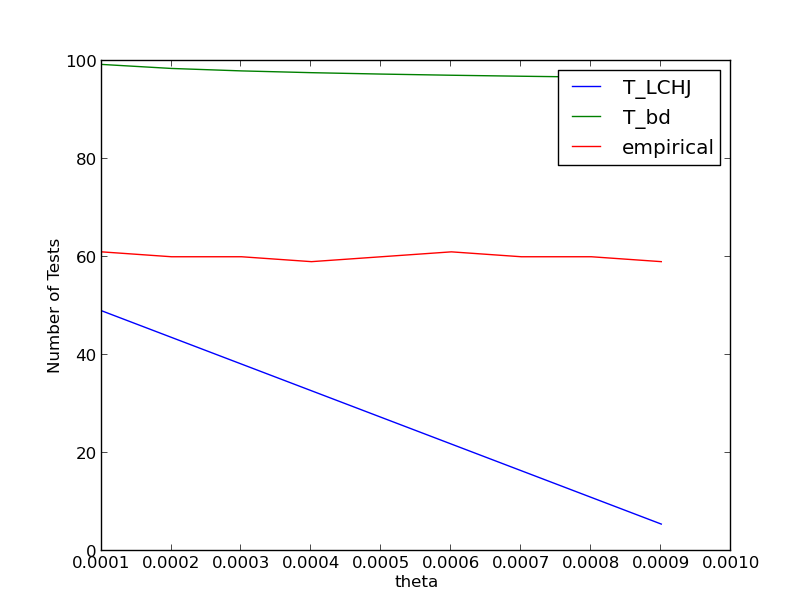
\includegraphics[width=0.5\textwidth]{ubvslb.png}
\caption{Theoretical lower and upper bounds and empirical Test frequencies as functions of \(\theta\)}
\label{ubvslb}
\end{figure}

Note that the Upper bound is not optimal and there still is some room for improvement. Note also that the lower bound degrades with \(\theta_i \). The lower bound (\(T_{LCHJ}\)) was generated according to Theorem (\ref{thm:upper}). 

\begin{figure}[h]
\centering
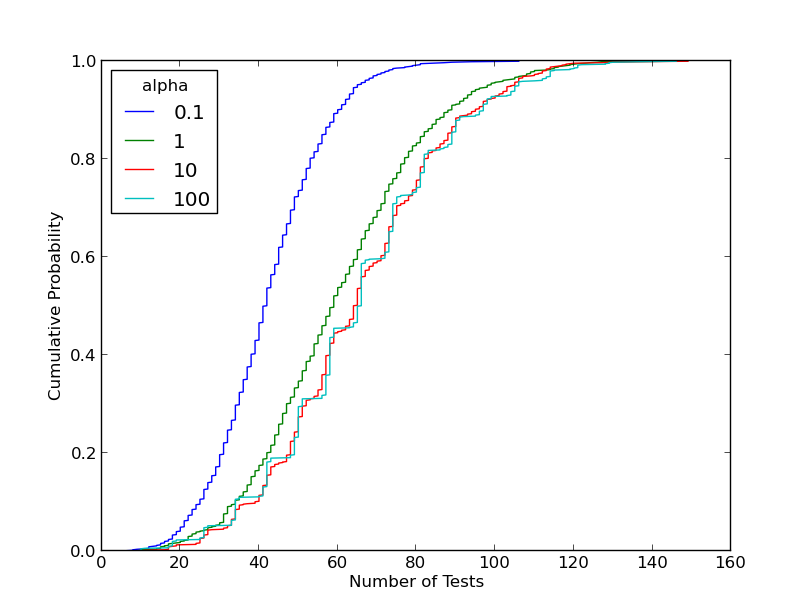
\includegraphics[width=0.5\textwidth]{variousalpha.png}
\caption{Cumulative distribution curves of the modified Hwang algorithm with fixed \(\theta = 0.0001\) and \(\alpha\) varying }
\label{testsvsalpha}
\end{figure}

\begin{figure}[h]
\centering
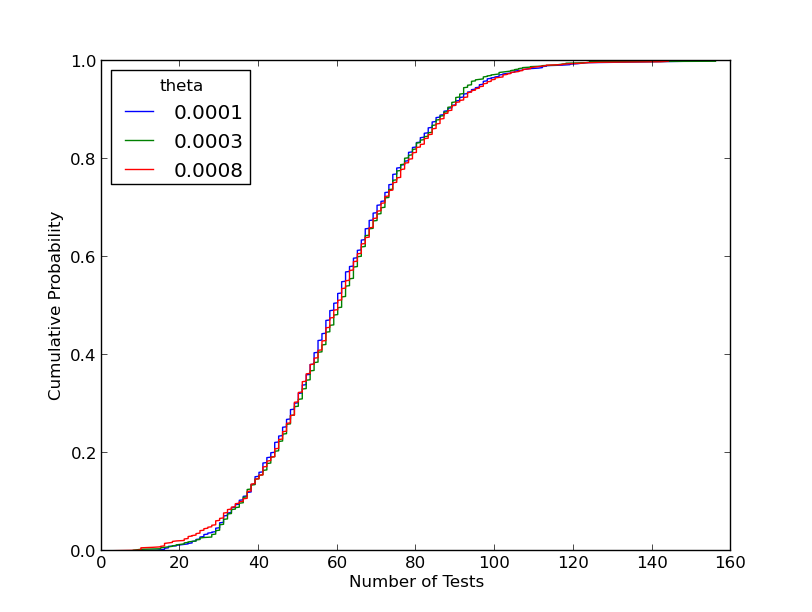
\includegraphics[width=0.5\textwidth]{nicegraphlaminar.png}
\caption{Cumulative distribution curves for fixed \(\alpha = 1\) and varying \(\theta\)}
\label{testsvstheta}
\end{figure}

Figures (\ref{testsvsalpha}) and (\ref{testsvstheta}) show that the performance is relatively insensitive to the cut-off \(\theta\), and more sensitive to the uniformity (or otherwise) of the probability distribution \(\vc{p}\). Heuristically, this is for because distributions which are highly concentrated on a few items algorithms can make substantial savings on the testing budget by testing those highly likely items first (which is captured in the bin structure of the above algorithm). 

The insensitivity to the cutoff \(\theta\) is due to items below \(\theta\) being overwhelmingly unlikely to be defective - which for small \(\theta\) means that few items (relative to the size of the problem) get discarded.

\section{Discussion}
%
We have introduced and analysed an algorithm for Probabilistic group testing which uses `just over' $H(\vc{U})$ tests to
recover all the defectives with high probability. Combined with a weak converse taken from \cite{li5}, this allows us to deduce that
the weak capacity of Probabilistic group testing is $C=1$.  
These results are illustrated by simulation.

For simplicity, this work has concentrated on establishing a bound $T_{\bd}$ in \eqref{eq:tbd} which has leading term $H(\vc{U})$,
and not on tightening bounds on the coefficient of $\mu$ in \eqref{eq:tbd}. For completeness, we mention that this coefficient
can be reduced from 3, under a simple further condition:

\begin{remark}
For some $c \leq 1/2$, we assume that all the $p_i \leq c$, and we alter the definition of `fullness' to assume that a set is
full if it has total probability less than $\alpha$. In this case, the term $P_{\setS} \log_2 P_{\setS}$ in \eqref{eq:tbds}
becomes $P_{\setS} \log_2 (\alpha + c)$, the bound in \eqref{eq:counting} becomes $\mu/\alpha$, and since
$\left( (1-p) \log_2 (1-p) \right)/p$ is decreasing in $p$, we can add a term $(1-c) \log_2 (1-c) $ to \eqref{eq:toopt}.
Overall, the coefficient of $\mu$ becomes $f(a,c) := \log_2 (\alpha + c) + 1 + 1/\alpha + (1-c) \log_2(1-c)$, which we can optimize over
$\alpha$. For example, if $c = 1/4$, taking $\alpha = 0.88824$, we obtain $f(a,c) = 2.00135$.
\end{remark}

It remains of interest to tighten the upper bound of Theorem \ref{thm:upper},
in order prove a strong converse, and hence confirm that the strong capacity is also equal to $1$.

In future work, we hope to explore more realistic models of defectivity, such as those where the defectivity of $U_i$ are not
necessarily independent, for example by imposing a Markov neighbourhood structure.

\section*{Acknowledgments}

This work was supported by the Engineering and Physical Sciences Research Council [grant number {\tt EP/I028153/1}]; Ofcom; and the University of Bristol. The authors would particularly like to thank Gary Clemo of Ofcom for useful discussions.
\chapter{Constrained Optimisation on Graphs}

\section{Introduction}

There is an almost ubiquitous growing demand for mobile and wireless data, with consumers demanding faster speeds and better quality connections in more places. Consequently 4G is now being rolled out in the UK and US and with 5G being planned for 2020 and beyond \cite{Dahlman2014}.  

However, there is constrained amount of frequencies over which to transmit this information; and demand for frequencies that provide sufficient bandwidth, good range and in-building penetration is high.

Not all spectrum is used in all places and at all times, and judicious spectrum management, by developing approaches to use white spaces where they occur, would likely be beneficial.

Broadly, access to spectrum is managed in two, complementary ways, namely through licensed and licence exempt access. Licensing authorises a particular user (or users) to access a specific frequency band. Licence exemption allows any user to access a band provided they meet certain technical requirements intended to limit the impact of interference on other spectrum users.

A licence exempt approach might be particularly suitable for managing access to white spaces. Devices seeking to access white spaces need a robust mechanism for learning of the frequencies that can be used at a particular time and location. One approach is to refer to a database, which maps the location of white spaces based on knowledge of existing spectrum users. An alternative approach is for devices to detect white spaces by monitoring spectrum use. 

The advantages of spectrum monitoring \cite{akan2009cognitive} over maintaining a database of space-frequency data are the ability of networks to make use of low-cost low-power devices, only capable of making local (as opposed to national) communications, keeping the cost of the network low and  opportunistic channel usage for bursty traffic, reducing channel collisions in dense networks.

The realisation of any Cognitive Radio standard (such as IEEE 802.22 \cite{stevenson2009ieee}), requires the co-existence of primary (e.g. TV users) and secondary (everybody else who wants to use TVWS spectrum) users of the frequency spectrum to ensure proper interference mitigation and appropriate network behaviour. We note, that whereas TVWS bands are an initial step towards dynamic spectrum access, the principles and approaches we describe are applicable to other frequency bands - in particular it makes ultra-wideband spectrum sensing possible.

The challenges of this technology are that Cognitive Radios (CRs) must sense whether spectrum is available, and must be able to detect very weak primary user signals. Furthermore they must sense over a wide bandwidth (due to the amount of TVWS spectrum proposed), which challenges traditional Nyquist sampling techniques, because the sampling rates required are not technically feasible with current RF or Analogue-to-Digital conversion technology.

Due to the inherent sparsity of spectral utilisation, Compressive Sensing (CS) \cite{Candes2006} is an appropriate formalism within which to tackle this problem. CS has recently emerged as a new sampling paradigm allowing images to be taken from a single pixel camera for example. Applying this to wireless communication, we are able to reconstruct sparse signals at sampling rates below what would be required by Nyquist theory, for example the works \cite{mishali2010theory}, and \cite{tropp2010beyond} detail how this sampling can be achieved. 

However, even with CS, spectrum sensing from a single machine will be costly as the proposed TVWS band will be over a large frequency range (for instance in the UK the proposed TVWS band is from 470 MHz to 790 MHz, requiring traditional sampling rates of \textasciitilde 600 MHz). CS at a single sensor would still require high sampling rates. In this report we propose a distributed model, which allows a sensing budget at each node far below what is required by centralised CS.

The contributions of this report are that we propose a distributed model and solver pair which obviates the need for a Fusion Centre (centralised node) as in \cite{Zhang2011b}) to do any data processing. That is the solution is found in a distributed manner, by local computations and communications in with one-hop neighbours. This can be applied to other models which previously required central processing.

Moreover, our algorithm is simple to understand (it is an extension of the multi-block ADMM \cite{mota2013d}) and can be applied to other composite optimisation problems.

We also give new proofs of ideas found in \cite{mota2013d}. 

The structure of the report is as follows: in section \ref{sec:sensingmodel} we introduce the sensing model, in section \ref{sec:opt-on-graphs} we describe the distributed reconstruction algorithm \cite{mota2013d}, and finally in section \ref{sec:results} we show some results of the reconstruction quality of this model. 

\section{ADMM}

Given a set of measurements of the form

\begin{equation}
y = Ax + n 
\end{equation}

where \(x \in \re^n\) is an \(s\)-sparse vector we wish to recover, \(y \in \re^m\) is a set of noisy measurements, \(A \in \re^{m \times n}\) is a design or measurement matrix s.t. \(x\) is not in the null-space of \(A\), and \(z \in \re^m\) is AGWN. The signal \(x\) can be recovered by algorithms minimising the objective function:

\begin{equation}
L = \frac{1}{2} \vectornorm{Ax-y}_2^2 + \lambda\vectornorm{x}_1
\label{LASSO}
\end{equation}

where \(\lambda\) is a parameter which trades off the reconstruction accuracy and sparsity of \(x\): larger \(\lambda\) means sparser \(x\). 

One such algorithm is the alternating direction method of multipliers \cite{Boyd2010a}, (ADMM). This algorithm solves problems of the form

\begin{align}
\argmin_{x} f\left( x \right) + g\left(z\right) \nonumber
\\
\text{s.t } Ux +Vz = c
\label{admm}
\end{align}

where \(f\) and \(g\) are assumed to be convex function with range in \(\re\), \(U \in \re^{p \times n}\) and \(V\in \re^{p \times m}\) are matrices (not assumed to have full rank), and \(c \in \re^p\).

ADMM consists of iteratively minimising the augmented Lagrangian 

\begin{align*}
L_p\left(x, z, \eta\right) = f\left( x\right) +& g\left(z\right)+\eta^T\left(Ux+Vz-c\right) + \frac{\rho}{2}\|Ux+Vz-c\|_2^2
\label{admm_form}
\end{align*}

(\(\eta\) is a Lagrange multiplier), and \(\rho\) is a parameter we can choose to make \(g(z)\) smooth \cite{nesterov2005smooth}, with the following iterations:

\begin{align}
x^{k+1} &:= \argmin_{x} L_\rho\left(x,z^k,\eta^k\right)\\
z^{k+1} &:= \argmin_{z} L_\rho\left(x^{k+1},z,\eta^k\right)\\
\eta^{k+1} &:= \eta^{k} + \rho \left(Ux^{k+1} + Vz^{k+1} - c\right)
\label{admm_algo}
\end{align}

The alternating minimisation works because of the decomposability of the objective function: the \(x\) minimisation step is independent of the \(z\) minimisation step and vice versa.  

We illustrate an example, relevant to the type of problems encountered in signal processing.

ADMM can be formulated as an iterative MAP estimation procedure for the problem \eqref{LASSO}. We can write \eqref{LASSO} in constrained form as:

\begin{eqnarray}
\frac{1}{2}\|Ax-b\|_2^2 + \lambda\|z\|_1 \\
\text{s.t } z = x
\end{eqnarray}

i.e this is of the form \eqref{admm} with \( f\left(x\right) =\|Ax-y\|_2^2\), \(g\left(z\right) = \lambda\|z\|_1\), \(U=I\), \(V=-I\), and \(c=0\).

The associated (augmented) Lagrangian is:

\begin{equation}
L_\rho = \frac{1}{2}\|Ax-b\|_2^2 + \lambda\|z\|_1 + \eta\left(x-z\right) + \frac{\rho}{2}\|x-z\|^2
\label{eq:lasso-lagrangian}
\end{equation}

The ADMM iterations for LASSO, which can be found by alternately differentiating \eqref{eq:lasso-lagrangian} with respect to \(x\),\(z\) and \(\eta\), are (in closed form):

\begin{align}
x^{k+1} &:= \left(A^TA + \rho I\right)^{-1}\left(A^Ty +\rho\left( z^k - \eta^k/\rho\right)\right)\\
z^{k+1} &:= S_{\lambda/\rho}\left(x^{k+1} + \eta^k/\rho\right)
 \\
\eta^{k+1} &:= \eta^{k} + \rho\left(x^{k+1}-z^{k+1}\right)
\label{admm_algo_lasso}
\end{align}

where \(S_{\lambda/\rho}\left(\circ\right)\) is the soft thresholding operator: \(S_\gamma\left(x\right)_i = \mathrm{sign}(x_i)\left(|x_i| - \gamma\right)^+\).

These can be found differentiating \eqref{eq:lasso-lagrangian} with respect to \(x\) and \(z\) as follows:

\begin{align*}
\frac{\partial L}{\partial x } = -A^T\left(y-Ax\right) + \rho (x-z) + \eta
\end{align*}

as 

\begin{equation}
\frac{\partial}{\partial x} \vectornorm{F(x)}_2^2 = 2\left(\frac{\partial}{\partial x} F(x)\right) F(x) 
\label{dellx}
\end{equation}

by the chain rule, and \(\partial/\partial x (Ax) = -A^T\) (see the Matrix Cookbook) as differentiation exchanges a linear operator with its adjoint.

Setting \eqref{dellx} to zero and collecting like terms:

\begin{equation}
\left(A^TA + \rho I\right)x = A^Ty + \rho z - \eta
\end{equation}

so we find the optimal \(x\) is:

\begin{equation}
x = \left(A^T A + \rho I\right)^{-1}\left(A^Ty + \rho \left( z - \eta/\rho\right)\right)
\label{optx}
\end{equation}

note that this estimator is a weighted average of the ordinary least squares estimate (\(A^Ty\)) and a Gaussian prior. This is to be expected, as the minimisation problem w.r.t x is an \(l_2\)-regularised MAP problem.

for \(z > 0\)

\begin{equation}
\frac{\partial L} {\partial z} = \lambda + \rho (x-z) - \eta
\label{dellz-positive}
\end{equation}

from which we obtain:

\begin{equation*}
z = x + \frac{1}{\rho} ( \eta - \lambda )
\end{equation*}

since \(z>0\) then \(x + \frac{1}{\rho} ( \eta - \lambda I) > 0\) when \(x + \frac{\eta}{\rho} > \frac{\lambda}{\rho}\).

Similarly for \(z < 0\):

\begin{equation}
\frac{\partial L} {\partial z} = -\lambda + \rho (x-z) 
\label{dellz-negative}
\end{equation}

setting \eqref{dellz-negative} to zero we obtain:

\begin{equation*}
z = x + \frac{1}{\rho}(\eta + \lambda)
\end{equation*}

since \(z<0\) then \(x + \frac{1}{\rho} ( \eta + \lambda ) < 0\) when \(x + \frac{\eta}{\rho} < - \frac{\lambda}{\rho}\).

at \(z=0\) we find:

\begin{equation*}
-\frac{\lambda}{\rho} \leq x + \frac{\eta}{\rho} \leq \frac{\lambda}{\rho}
\end{equation*}

i.e.

\begin{equation}
\mid x+ \frac{\eta}{\rho}\mid \leq \frac{\lambda}{\rho}
\label{zbounds}
\end{equation}

combining \eqref{dellz-negative}, \eqref{dellz-positive}, \eqref{zbounds} together we find the optimal \(z\) is:

\begin{equation}
z = \mathrm{sign}(x+\frac{\eta}{\rho})\text{ }\mathrm{max}\left( \mid x+\frac{\eta}{\rho} \mid - \frac{\lambda}{\rho} ,0\right)
\label{optz}
\end{equation}

Together \eqref{optx}, \eqref{optz} and the third step of \eqref{admm_algo_lasso} constitute the steps of the ADMM algorithm.

This algorithm has a nice statistical interpretation: it iteratively performs ridge regression, followed by shrinkage towards zero. This is the MAP estimate for \(x\) under a Laplace prior.

The soft-thresholding operator can be derived by considering the MAP estimate of the following model:

\begin{equation}
y = x + w
\end{equation}

where \(x\) is some (sparse) signal, and \(w\) is additive white Gaussian noise. We seek

\begin{equation}
\hat{x} = \arg\max_x \pr_{x|y}{\left(x|y\right)}
\end{equation}

This can be recast in the following form by using Bayes rule, noting that the denominator is independent of \(x\) and taking logarithms:

\begin{equation}
\hat{x} = \arg\max_x \left[\log{\pr_{w}{\left(y-x\right)}}+\log{\pr{\left(x\right)}}\right]
\label{hatx}
\end{equation}

The term \(\pr_{n}{\left(y-x\right)}\) arises because we are considering \(x+w\) with \(w\) zero mean Gaussian, with variance \(\sigma_n^2\). So, the conditional distribution of \(y\) (given \(x\)) will be a Gaussian centred at \(x\).

We will take \(\pr{\left(x\right)}\) to be a Laplacian distribution:

\begin{equation}
\pr{\left(x\right)} = \frac{1}{\sqrt{2}\sigma}\exp{-\frac{\sqrt{2}}{\sigma}|x|}
\end{equation}

Note that \( f\left(x\right) = \log{\pr_x{ \left( x \right)}} ~ -\frac{\sqrt{2}}{\sigma} |x| \), and so by differentiating \( f'\left(x\right) = -\frac{\sqrt{2}}{\sigma} \mathrm{sign}\left(x\right) \)

Taking the maximum of \ref{hatx} we obtain:

\begin{equation}
\frac{y-\hat{x}}{\sigma^2_n}-\frac{\sqrt{2}}{\sigma}sign(x) = 0
\end{equation}

Which leads the soft thresholding operation defined earlier, with \(\gamma = \frac{\sqrt{2}\sigma^2_n}{\sigma}\) as (via rearrangement):

$$
y =  \hat{x} + \frac{\sqrt{2}\sigma^2_n}{\sigma}\mathrm{sign}\left(x\right)
$$

or

$$
\hat{x}\left(y\right) = \mathrm{sign}(y)\left(y - \frac{\sqrt{2}\sigma^2_n}{\sigma}\right)_+
$$

i.e \(S_\gamma(y)\).

\subsection{The Proximity Operator}
The Proximity Operator for a closed, convex, and proper function \(f\) (the set of all such functions will be denoted \(\Gamma\) in a Hilbert space \(\mathcal{H}\) is defined as:

\begin{definition}[Proximity Operator]
\begin{equation}
\mathrm{Prox}_f\left(y\right) :=  \argmin_{y \in \mathcal{H} } f\left(y\right) + \frac{1}{2}\vectornorm{y-x}^2
\end{equation}
\end{definition}

Intuitively the Proximity Operator approximates a point \(x\) by another point \(y\), that is close in the mean-square sense under the penalty \(f\).

The \(\mathrm{Prox}\left(\circ\right)\) operator exists for closed and convex \(f\) as \(\left(y\right) + \frac{1}{2}\vectornorm{y-x}^2\) is closed with compact level sets and is unique as \(\left(y\right) + \frac{1}{2}\vectornorm{y-x}^2\) is strictly convex.

The corresponding Moreau envelope is defined as 

\begin{definition}[Moreau Envelope]
\begin{equation}
\mathrm{M}_f\left(y\right) :=  \min_{y \in \mathcal{H}} f\left(y\right) + \frac{1}{2}\vectornorm{y-x}^2
\end{equation}
\end{definition}

The Moreau envelope is a strict generalisation of the squared distance function. \(\mathrm{M}_f\) is real valued - even when \(f\) takes the value \(\infty\), whilst \(\mathrm{Prox}_f \) is \(\mathcal{H}\)-valued. 

\subsubsection{Properties}
\begin{theorem}[Moreau '65]
Let \(f \in \Gamma\) and \(f^*\) be its Fenchel conjugate. Then the following are equivalent:
\begin{itemize}
\item \(z = x+y, y \in \partial f\left(x\right)\)
\item \(x = \mathrm{Prox}_f\left(z\right), y = \mathrm{Prox}_{f^*}\left(z\right)  \)
\end{itemize}
\end{theorem}

\begin{theorem}[Moreau '65]
Let \(f \in \Gamma\). Then for all \(z \in \mathcal{H}\)
\begin{itemize}
\item \( \mathrm{Prox}_f\left(z\right) + \mathrm{Prox}_{f^*}\left(z\right) = z   \)
\item \( \mathrm{M}_f\left(z\right)  + \mathrm{M}_{f^*}\left(z\right)  = \frac{1}{2}\vectornorm{z}^2 \)
\end{itemize}
\end{theorem}

\begin{theorem}[Moreau '65]
The Moreau envelope is (Frechet) differentiable, with 
\begin{equation}
\nabla \mathrm{M}_f = Id - \mathrm{Prox}_{f} = \mathrm{Prox}_{f^*}
\end{equation}
\end{theorem}

\begin{theorem}[Moreau '65]
\( \mathrm{Prox}_f : \left(\mathcal{H}, \vectornorm{\circ}\right) \leftarrow \left(\mathcal{H}, \vectornorm{\circ}\right) \) is 1-Lipchitz continuous.
\end{theorem}

\subsubsection{Motivation}
We are solving problems of the following form:

\begin{align}
&\min_{x \in \mathcal{H}} f\left(x\right) + g\left(z\right)\\
&\text{s.t } x - z = 0
\end{align}

with \(f, g \in \Gamma\). To solve this problem we form the augmented Lagrangian: 

\begin{align*}
L_p\left(x, z, \eta\right) = f\left( x\right) +& g\left(z\right)+\eta^T\left(Ux+Vz-c\right) + \frac{\rho}{2}\|Ux+Vz-c\|_2^2
\end{align*}

and then performing the following iterative minimisation:

\begin{align}
x^{k+1} &:= \argmin_{x} L_\rho\left(x,z^k,\eta^k\right)\\
z^{k+1} &:= \argmin_{z} L_\rho\left(x^{k+1},z,\eta^k\right)\\
\eta^{k+1} &:= \eta^{k} + \rho \left(x^{k+1} + z^{k+1}\right)
\end{align}

i.e. 

\begin{align}
x^{k+1} &:= \argmin_{x} \left( f\left(x\right) + \eta^{kT}x + \frac{\rho}{2}\vectornorm{x - z^k}^2 \right) \\
z^{k+1} &:= \argmin_{z} \left( g\left(z\right) - \eta^{kT}z + \frac{\rho}{2}\vectornorm{x^{k+1} - z}^2 \right)\\
\eta^{k+1} &:= \eta^{k} + \rho \left(x^{k+1} + z^{k+1}\right)
\end{align}

pulling the linear terms into the quadratic ones we get:

\begin{align}
x^{k+1} &:= \argmin_{x} \left( f\left(x\right) +  \frac{\rho}{2}\vectornorm{x - z^k + \left(1/\rho\right)\eta^k}^2 \right) \\
z^{k+1} &:= \argmin_{z} \left( g\left(z\right) +  \frac{\rho}{2}\vectornorm{x^{k+1} - z - \left(1/\rho\right)\eta^k}^2 \right)\\
\eta^{k+1} &:= \eta^{k} + \rho \left(x^{k+1} + z^{k+1}\right)
\end{align}

i.e.

\begin{align}
x^{k+1} &:= \mathrm{Prox}_f \left( z^k - u^k\right)\\
z^{k+1} &:= \mathrm{Prox}_f \left(x^{k+1} + u^k\right)  \\
u^{k+1} &:= u^{k} + \left(x^{k+1} + z^{k+1}\right)
\end{align}

with \(u^k = \left(1/\rho\right) \eta^k\).

The motivation for the Proximal operator should now be clear: to perform the minimisation we simply calculate the proximal operator of each of the functions at each step. For many functions found in Statistics (e.g. the \(l_p\) norms, this can be found in closed form, and so ADMM presents a particularly attractive method for finding MAP solutions to regularised statistical problems.

\subsubsection{Examples}

\begin{example}[Indicator]
From the definition 

\begin{align}
\mathrm{Prox}_I\left(x\right) &:=  \argmin_y I_C(y) + \frac{1}{2}\vectornorm{y-x}^2 \\
& = \argmin_{y \in C} \frac{1}{2}\vectornorm{y-x}^2 \\
& = P_C\left(x\right)
\end{align}

where \(I_C(y)\) is the indicator of some set \(C\) and \(P_C\) is the projection operator onto that set.
\end{example} 

\begin{example}[\(l_2\) norm]
For \(f(y) = \frac{\mu}{2}\vectornorm{y}^2\) the \(\mathrm{Prox}\) operator is:

\begin{align}
\mathrm{Prox}_f\left(x\right) &:=  \argmin_y \frac{\mu}{2}\vectornorm{y}^2 + \frac{1}{2}\vectornorm{y-x}^2 \\
& = \frac{1}{1+\mu}x
\end{align}
\end{example}

\begin{example}[\(l_1\) norm]
\(f = \|x\|_1\)

\begin{equation}
\mathrm{Prox}_f\left(x\right) := \mathrm{sign}(x_i)\left(|x_i| - \gamma\right)^+ = S_\gamma\left(x\right)_i 
\end{equation}
\end{example}

\begin{example}[Elastic Net]
Consider

\begin{equation}
f(x) = \lambda\|x\|_1 + \mu \vectornorm{x} 
\end{equation}

\begin{equation}
\mathrm{Prox}_f\left(x\right) := \frac{\lambda}{1+\mu} S_\gamma\left(x\right)_i 
\end{equation}
\end{example}

\begin{example}[Fused Lasso]
Consider

\begin{equation}
f(x) = \|x\|_1 + \sum_{i=1}^{d-1} \left( x_i - x_{i-1} \right) 
\end{equation}

i.e the sum of the \(l_1\) and \(TV\) norms

\begin{equation}
\mathrm{Prox}_f\left(x\right) := \mathrm{Prox}_{l_1} \circ \mathrm{Prox}_{TV} =  S_\gamma\left(\mathrm{Prox}_{TV}\right)_i 
\end{equation}
\end{example}

\begin{example}[Consensus]

Suppose we want to solve a problem such as:

\begin{equation*}
\begin{aligned}
& \underset{x}{\text{minimize}}
& & \sum_i f_i\left( x \right) \\
\label{consensus}
\end{aligned}
\end{equation*}

this could arise in statistical computing where \(f_i\) would be the loss function for the \(i^th\) block of training data. We can write the problem for distributed optimisation as:

\begin{equation*}
\begin{aligned}
& \underset{x}{\text{minimize}}
& & \sum_i f_i\left( x_i \right) \\
& \text{subject to}
& & x_i - z = 0
\label{admm_consensus}
\end{aligned}
\end{equation*}

where \(x_i\) are local variables (for example local to each node in a spectrum sensing) and \(x_i - z = 0\) are the consensus constraints. Consensus and regularisation can be achieved by adding a regularisation term \(g\left(z\right)\) - for example \(g\left(z\right) = \lambda||x||_1\) corresponds to the LASSO, and the \(f_i\) would be \(f_i = ||A_ix_i - b||_2^2\). 

As per the previous sections, we form the Augmented Lagrangian:

\begin{equation}
L_\rho\left(x,y\right) = \sum_i^n \left(f_i\left( x_i \right) + y_i^T\left(x_i-z\right) + \frac{\rho}{2}\|x_i-z\|_2^2\right)
\end{equation}

The ADMM iterations for this Lagrangian are:

\begin{align}
x_i^{k+1} &:= \argmin{x_i} \left(f_i\left( x_i \right) + y_i^{kT}\left(x_i-z\right) + \frac{\rho}{2}\|x_i-z\|_2^2\right)\\
z^{k+1} &:= \frac{1}{n}\sum_i^n \left(x_i^{k+1} + \left(1\rho\right)y_i^k\right)\\
y_i^{k+1} &:= y_i^{k} + \rho \left(x_i^{k+1} - z^{k+1} \right)
\label{consensus_iterations}
\end{align}

The \(z^{k+1}\) iteration is analytic as we're minimising the squared norm of \(x_i - z\) - so we average. With \(\|x\|_1\) regularisation we perform soft-thresholding after the \(z\) update.

At each iteration the sum of the dual variables \(y_i\) is zero, so the algorithm can be simplified to:

\begin{align}
x_i^{k+1} &:= \argmin{x_i} \left(f_i\left( x_i \right) + y_i^{kT}\left(x_i-\bar{x}^k\right) + \frac{\rho}{2}\|x_i-\bar{x}^k\|_2^2\right)\\
y_i^{k+1} &:= y_i^{k} + \rho \left(x_i^{k+1} - z^{k+1} \right)
\label{simple_consensus_iterations}
\end{align}
 
where

\begin{equation}
\bar{x}^k = \frac{1}{n} \sum_i^n x_i^k
\end{equation}

This algorithm can be summarised as follows: in each iteration

\begin{itemize}
\item gather \(x^k\) and average to get \(\bar{x}^k\)
\item scatter the average to nodes
\item update \(y_i^k\) locally
\item update \(x_i\) locally
\end{itemize}

Each agent is minimising it's own function, plus a quadratic term (the squared norm) which penalises the agent from moving too far from the previous average.

Note that the 'gather' stage doesn't require a central processor - this can be done in a distributed manner also.
\end{example}

\subsection{Statistical Interpretation}
At each step \(k\) of the algorithm each agent is minimising it's own loss function, plus a quadratic.
This has a simple interpretation: we're doing MAP estimation under the prior \(\mathcal{N}\left(\bar{x}^{k} + \left(1\rho\right)y_i^k, \rho I\right)\). I.e. the prior mean is the previous iteration's consensus shifted by node \(i\) disagreeing with the previous consensus. 

\subsection{Acceleration}


\section{Constrained Optimisation on Graphs}\label{sec:opt-on-graphs}

We model the network of sensors as an undirected graph \(G = \left(V,E\right)\), where \(V = \{1 \ldots J\}\) is the set of vertices, and \(E = V \times V\) is the set of edges. An edge between nodes \(i\) and \(j\) implies that the two sensors can communicate. The set of nodes that node \(i\) can communicate with is written \(\mathcal{N}_i\) and the degree of node \(i\) is \(D_i = |\mathcal{N}_i|\). 

Individually nodes make the following measurements (as discussed in section \ref{sec:sensingmodel}):

\begin{equation}
\vec{y}_p = \vec{A}_p\vec{x} + \vec{n}_p
\end{equation}

where \(\vec{A}_p\) is the \(p^{th} \) row of the sensing matrix from \eqref{system}, and the system \eqref{system} is formed by concatenating the individual nodes' measurements together.

We assume that a proper colouring of the graph is available: that is, each node is assigned a number from a set \(C = \{1 \ldots c \} \), and no node shares a colour with any neighbour. This is so that nodes may communicate in colour order, as opposed to communicating individually thus reducing the total number of communication rounds required. 

To find the \(\vec{x}\) we are seeking (the solution to the linear system, \ref{system}), to each node we give a copy of \(\vec{x}, \vec{x}_p\) and we constrain the copies to be identical across all edges in the network. Each node, thus has a separate optimisation to solve, subject to the constraint that it is consistent with its neighbours.

The problem then is to solve:

\begin{align}
\argmin_{\bar{x}} \sum_{c=1}^C \sum_{j \in c} f\left(x_j\right) + \frac{\lambda}{J} g\left(x_j\right) \nonumber \\ 
\text{ and } x_i = x_j \text{ if } \{i,j\} \in E \nonumber \\
\text{ and } x_i = z_i \text{ } \forall i \in \{1, \ldots, C\}
\label{constrainedbp}
\end{align}

with a particular special case being:

\begin{align}
\argmin_{\bar{x}} \sum_{c=1}^C \sum_{j \in c} \|A_jx_j - y_j\|_2^2 + \frac{\lambda}{J}\|z\|_1 \nonumber \\ 
\text{ and } x_i = x_j \text{ if } \{i,j\} \in E \nonumber \\
\text{ and } x_i = z_i \text{ } \forall i \in \{1, \ldots, C\}
\label{constrainedbp}
\end{align}

i.e. \(f = \vectornorm{x}_2^2\) and \(g = \vectornorm{x}_1\).

That is, at each node we minimise a Lasso functional constrained to be consistent across edges but that is separable in the \(l_2\) and \(l_1\) norms.

We can write the global optimisation variable as \(\bar{x}\), which collects together \(C\) copies of a \(n\times 1\) vector \(\vec{x}\):

\begin{defn}
We define vectors \(x_c\), where \(c = 1,\ldots , C\) and write the vector of length \(nJ\):
\begin{equation}
\bar{x} = \sum_{c=1}^C w_c \otimes x_c = \left[x_{c(1)}^T, \ldots	, x_{c(J)}^T\right]^T
\label{barxc}
\end{equation}
where \(w_{c(i)} = \mathbb{I}(c(i) = c)\), \(\mathbb{I}\) is the indicator function, and we have written \(c(i)\) for the colour of the \(i\)th node.
\end{defn}

These constraints can be written more compactly by introducing the node-arc incidence matrix B: a \(V\) by \(E\) matrix where each column is associated with an edge \(\left(i,j\right) \in E\) and has \(1\) and \(-1\) in the \(ith\) and \(jth\) entry respectively. Figures \eqref{efig:ex-network} and \eqref{fig:incidence-matrix} show examples of a network and it's associated incidence matrix.

The constraint \(x_i = x_j \text{ if } \{i,j\} \in E \) can now be written 

\begin{equation}
\sum_{c=1}^C\left(B_c^T \otimes I_n\right)\bar{x}_c = 0
\label{compact-constraints}
\end{equation}

note that \(\left(B^T\otimes I_n \right) \in \re^{nE \times nJ}\). Together \eqref{barxc} and \eqref{compact-constraints}, suggests that the problem \eqref{constrainedbp} can be re-written as:

\begin{align}
\argmin_{\bar{x}} \sum_{c=1}^C \sum_{j \in C_c} f\left(x_j\right) + \frac{\lambda}{J} g\left(z_j\right)
\nonumber \\
\text{ s.t. } \sum_{c=1}^C\left(B_c^T \otimes I_n\right)\bar{x}_c = 0 \nonumber \\
\text{ and } \bar{x}_c - \bar{z}_c = 0
\label{constrainedbp1}
\end{align}

where \(\beta = \frac{\lambda}{J}\).

The global Augmented Lagrangian \cite{Boyd2010a}
 for the problem \eqref{constrainedbp1} can be written down as:

\begin{align}
L_\rho = \sum_{c=1}^C  ( \sum_{j \in c} & f\left(x_j\right) + \frac{\lambda}{J} g\left(z_j\right)  + \nonumber \\ & + \theta^T\left(\bar{x}_j - \bar{z}_j\right)  +  \frac{\rho}{2}\vectornorm{\bar{x}_j-\bar{z}_j}_2^2 ) + \nonumber \\  & + \eta^T\left(B_c^T \otimes I_n\right)\bar{x}_c + \frac{\rho}{2}\vectornorm{\sum_{c=1}^C\left(B_c^T \otimes I_n\right)\bar{x}_c}_2^2
\label{aug-lagrange}
\end{align}

This is, superficially, similar to the Augmented Lagrangian for the Lasso problem \cite{Boyd2010a}[Section 6.4]. That is, the terms indexed by \(j\) are a straightforward Lasso problem, constrained by edge-wise variables (indexed by \(c\)) forcing consistency across the network. However, the problem (as currently written) is not separable across the edges of the network as the final and penultimate term represent the constraint that the nodes agree on their estimates across edges. 

To make it possible that \ref{aug-lagrange} can be posed  as a constrained optimisation problem at each node, we introduce the following variable (so that the the final term of \ref{aug-lagrange} is separable across edges of the graph):

\begin{defn}
\begin{align*}
u &:= \left(B^T \otimes I_n\right)\bar{x} \\
& = \left(B^T \otimes I_n\right)\sum_{c=1}^C w_c \otimes x_c \\
& = \sum	_{c=1}^C B_c^T\otimes x_c
\end{align*}
where we have used the definition \eqref{barxc} in the second line, and the property of Kronecker products \((A\otimes C)(B \otimes D) = (AB \otimes CD)\) between the second and third lines, and we write \(B_c = w_c^TB\).
\end{defn}

\begin{figure}[h]
\centering
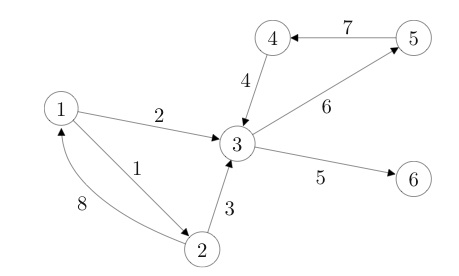
\includegraphics[height = 5 cm]{network-ex-incidence-mat.jpg}
\caption{An example of a network}
\label{efig:ex-network}
\end{figure}

\begin{figure}[h]
\centering
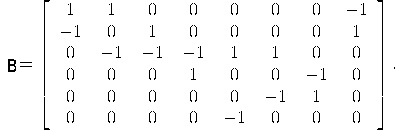
\includegraphics[height = 3 cm, width = 7cm]{ex-incidencematrix1.png}
\caption{The incidence matrix associated with Figure \eqref{efig:ex-network}}
\label{fig:incidence-matrix}
\end{figure}

The terms \(\|\sum_{c=1}^C\left(B_c^T \otimes I_n\right)\bar{x}_c\|^2\) and \( \eta^T\left(B_c^T \otimes I_n\right)\bar{x}_c \) of \eqref{aug-lagrange}, can be decomposed across edges, using the following lemma:

\begin{lemma}[Edge Decomposition]
\begin{equation}
\vectornorm{\sum_{c=1}^C\left(B_c^T \otimes I_n\right)\bar{x}_c}^2 = \sum_{j \in C_1}\left( D_j\vectornorm{x_j}_2^2 - \sum_{k \in N_j} x_j^Tx^k\right)
\end{equation}

and

\begin{equation}
\eta^T\sum_{c=1}^C\left(B_c^T \otimes I_n\right)\bar{x}_1 = \sum_{l\in C_c} \sum_{m\in N_l}sign\left(m-l\right)\eta_{ml}^T x_l
\end{equation}

where \(\eta\) is decomposed edge-wise: \(\eta = \left(\ldots, \eta_{ij},\ldots\right)\), such that \(\eta_{i,j} = \eta_{j,i}\), and is associated with the constraint \(x_i = x_j\).


\begin{proof}

\begin{align*}
u^Tu &= \sum	_{c_1=1}^C \sum	_{c_2=1}^C  \left(B_{c_1} \otimes x_{c_1}^T\right) \left(B_{c_2}^T \otimes x_c\right) \\
&= \sum_{c_1, c_2} B_{c_1}B_{c_2}^T \otimes x_{c_1}^Tx_{c_2}
\end{align*}

\(BB^T\) is a \(J \times J\) matrix, with the degree of the nodes on the main diagonal and \(-1\) in position \(\left(i,j\right)\) if nodes \(i\) and \(j\) are neighbours (i.e \(BB^T\) is the graph Laplacian). Hence, since we can write \(B_{c_1}B_{c_2}^T = w_{c_1}^TBB^Tw_{c_2}\), the trace of \(B_{c_1}B_{c_1}^T\) is simply the sum of the degrees of nodes with colour 1. 

For \(c_1 \neq c_2\),  \(B_{c_1}B_{c_2}^T\) corresponds to an off diagonal block of the graph Laplacian, and so counts how many neighbours each node with colour 1 has.

Finally, note that \(\eta \in \re^{nE}\) and can be written:

\begin{equation}
\eta = \sum_{c=1}^C w_c \otimes \eta_c
\end{equation}
where \(\eta_c\) is the vector of Lagrange multipliers associated across edges from colour \(c\). Now

\begin{align*}
\eta^Tu = \sum_{c_1=1}^C\sum_{c_2=1}^C w_{c_1}Bw_{c_2} \otimes \eta_{c_1}^Tx_c
\end{align*}
by the properties of Kronecker products, and the definition of \(B_c\). For \(c_1=c_2\), \(\eta^Tu\) is zero, as there are no edges between nodes of the same colour b definition. For \(c_1\neq c_2\), \(\eta^Tu\) counts the edges from \(c_1\) to \(c_2\), with the consideration that the edges from \(c_2\) to \(c_1\) are counted with opposite parity.
\end{proof}
\end{lemma}



Adding together this with the lemma, lets us write \eqref{aug-lagrange} as:

\begin{align}
L_\rho = \sum_{c=1}^C\sum_{j \in C_c} &\left( f\left(x_j\right) + \beta g\left(z_j\right)\right) + \nu^Tx_j \nonumber \\
& \text{        } \theta\left(x_j - z_j\right) + \frac{\rho}{2}D_i\vectornorm{x_j}^2 + \frac{\rho }{2}\|x_j-z_j\|^2
\label{generic-iterations}
\end{align}

where we have defined:

\begin{equation}
\nu_i = \left(\sum_{k \in \mathcal{N}_i} sign\left(k-i\right)\eta_{\{i,k\}} - \rho x_k \right)
\end{equation}

this is a rescaled version of the Lagrange multiplier, \(\eta\), which respects the graph structure. 

Then by differentiating \eqref{generic-iterations} with respect to \(x_j\) and \(z_j\) we  can find closed forms for the updates as:

\begin{thm}
\begin{align}
x_j^{k+1} &:= \left(A_j^TA_j + (\rho D_J + 1) I\right)^{-1}\left(A_j^Ty_j +  z^k - \nu^{kT}\right)\\
z_j^{k+1} &:= S_{\beta/\rho}\left(x_j^{k+1} \right)
 \\
\theta_j^{k+1} &:= \theta_j^{k} + \rho \left(x^{k+1}-z^{k+1}\right) \\
\eta_j^{k+1} &:= \eta_j^k + \rho\left(\sum_{m \in N_j} z_m^k - z_j^k\right)
\label{dadmm_algo_lasso}
\end{align}
\end{thm}

This algorithm can be thought of as follows: each node performs an iteration of (non multi-block) ADMM - i.e. each node solves an approximate Gaussian least-squares problem and then soft-thresholds - and then exchanges the result of this computation with its one-hop neighbours. This explains the inclusion of an extra Lagrange multiplier: the multiplier \(\theta\) controls how far each node moves from its previous estimate in each iteration, whilst the multiplier \(\eta\) enforces consistency between nodes. Note that there is no communication of data between the nodes - only the result the computation in each round.
 %\input{Chapters/Chapter3}
\chapter{Compressive Sensing Architechtures}\label{sec:sensingmodel}

\subsection{Modulated Wideband Converter}
We consider a radio environment with a single primary user (PU) and a network of \(J\) nodes collaboratively trying to sense and reconstruct the PU signal, either in a fully distributed manner (by local communication), or by transmitting measurements to a fusion centre which then solves the linear system. 

We try to sense and reconstruct a wideband signal, divided into \(L\) channels. We have a (connected) network of \(J\) (= 50) nodes placed uniformly at random within the square \(  \left[0,1\right]\times \left[0,1\right] \). This is the same model, as in \cite{Zhang2011b}. The calculations which follow are taken from \cite{Zhang2011b} as well.

The nodes individually take measurements (as in \cite{mishali2010theory}) by mixing the incoming analogue signal \(x\left(t\right)\) with a mixing function \(p_i\left(t\right)\) aliasing the spectrum. \(x\left(t\right)\) is assumed to be bandlimited and composed of up to \(k\) uncorrelated transmissions over the \(L\) possible narrowband channels - i.e. the signal is \(k\)-sparse. 

\begin{figure}[h]
\centering
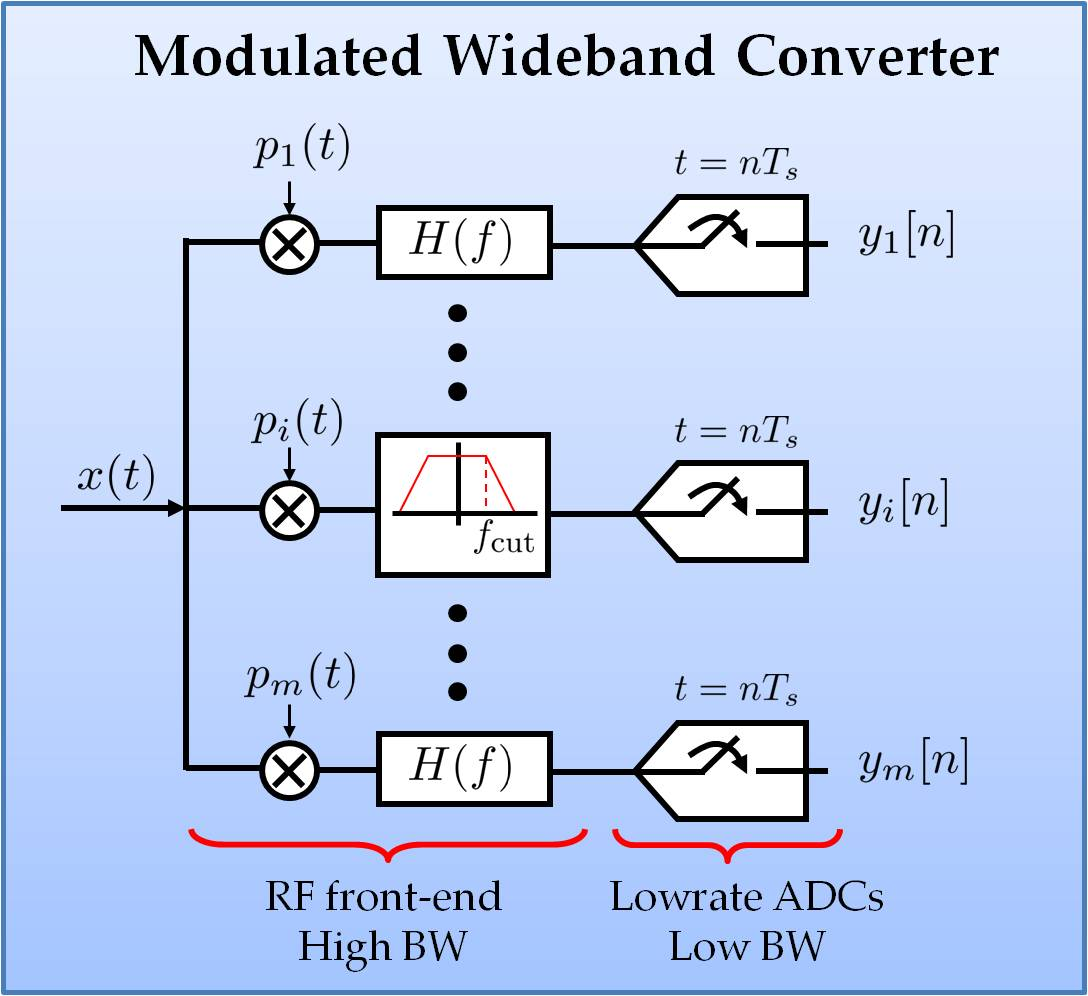
\includegraphics[height = 7.3 cm]{Modulated_wideband_converter.jpg}
\caption{Mse vs SNR for the sensing model, with AWGN only, showing the performance of distributed and centralised solvers}
\label{msevssnr0}
\end{figure}

The mixing functions - which are independent for each node - are required to be periodic, with period \(T_p\). Since \(p_i\) is periodic it has Fourier expansion:

\begin{equation}
p_i\left(t\right) = \sum_{l=-\infty}^{\infty} c_{il} \exp\left({jlt\frac{2\pi}{T_p}}\right)
\end{equation}

The \(c_{il}\) are the Fourier coefficients of the expansion and are defined in the standard manner. The result of the mixing procedure in channel \(i\) is therefore the product \(xp_i\), with Fourier transform (we denote the Fourier Transform of \(x\) by \(X\left( \dot{.} \right)\)):

\begin{align}
X_{i}\left(f\right) &=& \int_{-\infty}^{\infty} x\left(t\right) p_i\left(t\right) dt \nonumber
\\ &=& \sum_{l=-\infty}^{\infty} c_{il} X\left(f-lf_p\right)
\end{align}

(We insert the Fourier series for \(p_i\), then exchange the sum and integral). The output of this mixing process then, is a linear combination of shifted copies of \(X\left(f\right)\), with at most \(\lceil f_NYQ/f_p\rceil\) terms since \(X\left(f\right)\) is zero outside its support (we have assumed this Nyquist frequency exists, even though we never sample at that rate).

This process is repeated in parallel at each node so that each band in \(x\) appears in baseband.

Once the mixing process has been completed the signal in each channel is low-pass filtered and sampled at a rate \(f_s \geq f_p\). In the frequency domain this is a ideal rectangle function, so the output of a single channel is:

\begin{equation}
Y_i\left(e^{j 2 \pi f T_s }\right) = \sum_{l = -L_0}^{+L_0} c_{il} X\left(f-lf_p\right)
\end{equation}

since frequencies outside of \([-f_s/2, f_s/2]\) will filtered out. \(L_0\) is the smallest integer number of non-zero contributions in \(X\left(f\right)\) over \([-f_s/2, f_s/2]\) - at most \(\lceil f_NYQ/f_p\rceil\) if we choose \(f_s = f_p\). These relations can be written in matrix form as:

\begin{equation}
\textbf{y} = \textbf{A}\textbf{x} + \vec{w}
\label{system}
\end{equation}

where \(\textbf{y}\) contains the output of the measurement process, and \(\textbf{A}\) is a product matrix of the mixing functions, their Fourier coefficients, a partial Fourier Matrix, and a matrix of channel coefficients. \(\textbf{x}\) is the vector of unknown samples of \(x\left(t\right)\). 

i.e. \(\textbf{A}\) can be written: 

\begin{equation}
\textbf{A}^{m\times L} = \textbf{S}^{m\times L} \textbf{F}^{L\times L} \textbf{D}^{L \times L} \textbf{H}^{L \times L}
\end{equation}

The system  \ref{system} can then be solved (in the sense of finding the sparse vector \(\vec{x}\) by convex optimisation via minimising the objective function:

\begin{equation}
\frac{1}{2}\|\textbf{Ax}-\textbf{y}\|_2^2 + \lambda \|\textbf{x}\|_1
\end{equation}

where \(\lambda\) is a parameter chosen to promote sparsity. Larger \(\lambda\) means sparser \(\vec{x}\).

\subsection{Random Demodulator}
We assume that the analogue signal \(x\left(t\right)\) is comprised of a finite number of components from some arbitrary dictionary \(\psi_n\left(t\right)\):

\begin{equation}
x\left(t\right) = \sum_{n=1}^N \alpha_n \psi_n\left(t\right)
\end{equation}

The signal is said to be sparse when there are only a few non-zero \(\alpha_n\). The dictionary elements \(\psi_n\) may have a relatively high bandwidth, but the signal itself will have only a few degrees of freedom.

The signal acquisition method proposed consists of three stages (all analogue processing): demodulation, filtering and uniform sampling. 

Initially, the signal is modulated by a pseudo-random sequence \(p_c\left(t\right)\), which alternates at frequencies at (or above) the Nyquist frequency of \(x\left(t\right)\). The signal is then filtered, through a filter with impulse response \(h\left(t\right)\), before being sampled at rate \(\mathcal{M}\) with a traditional ADC.

The output of this system, \(y\left[m\right]\), can be related to the input \(x\left(t\right)\) via a linear transformation of the coefficient vector \(\alpha_n\). 

To find the transformation \(A\), first consider the output of \(y\left[m\right]\), which is the result of convolution and demodulation followed by sampling at rate \(\mathcal{M}\):

\begin{equation}
y\left[m\right] = \int_{-\infty}^{\infty} x\left(\tau\right)p_c\left(\tau\right)h\left(t - \tau\right)\mid_{t = m\mathcal{M}}d\tau
\end{equation}

and by expanding \(x\left(t\right) = \sum_{n=1}^N \alpha_n \psi_n\left(t\right)\):

\begin{equation}
y\left[m\right] =  \sum_{n=1}^N \alpha_n \int_{-\infty}^{\infty} \psi_n\left(t\right)p_c\left(\tau\right)h\left(m\mathcal{M} - \tau\right)d\tau
\end{equation}

we see that the output can be written as:

\begin{equation}
y = Ax
\end{equation}

with

\begin{equation}
A_{m,n} = \int_{-\infty}^{\infty} \psi_n\left(t\right)p_c\left(\tau\right)h\left(m\mathcal{M} - \tau\right)d\tau
\end{equation}

\section{Joint Space-Frequency Model}
We write the power spectral density (psd) of the \(sth\) transmitter as:

\begin{equation}
\phi_s = \sum_b \beta_{bs} \psi_b\left(f\right)
\label{basis_expansion}
\end{equation}
\\ 

This model expresses in psd of the transmitter in a suitable basis - for example \(\psi_b\left(f\right)\) could be zero everywhere except for the set of frequencies where \(f=b\) i.e. \(\psi\) is a rectangular function with height \(\beta_{bs}\) and support \(f\). Other candidates for \(\psi\) include splines (e.g. raised cosines), and complex exponentials. 

Given this, the psd at the \(rth\) receiver is:

\begin{equation}
\phi_r = \sum_s g_{sr}\phi_s = \sum_s g_{sr} \sum _b \beta_{bs}\psi_b\left(f\right)
\end{equation}

where

\begin{equation}
g_{sr} = \exp\left(-||x_r - x_s||_2^\alpha\right)
\end{equation}

is the channel response between the \(sth\) transmitter and the \(rth\) reciver.

This model can be summarised using Kronecker products as follows:

Let \(\tilde{G} = g_sr^T\), \(e_r, e_b\) be unit vectors i.e. they are \(1\) for the \(i^{th}\) receiver or frequency band respectively.

The received power at a receiver (when only a single transmitter is transmitting) can be written:

\begin{equation}
y_r = \left(	e_r^T \bigotimes I_{n_b}\right) y
\end{equation}

with,

\begin{equation}
y = \left( \tilde{G} \bigotimes I_{n_b} \right) \phi
\end{equation}

Now, we have

\begin{equation}
\phi = e_s \bigotimes \phi_s
\end{equation}

so,

\begin{equation}
y = \left( \tilde{G} \bigotimes I_{n_b} \right) \left(e_s \bigotimes \phi_s \right)
\end{equation}

finally we have,

\begin{equation}
y_r = \left(	e_r^T \bigotimes I_{n_b}\right)\left[\left( \tilde{G} \bigotimes I_{n_b} \right) \left(e_s \bigotimes \phi_s \right)\right]
\end{equation}

\(\beta_{bs} \in \re^{1 \times n_b}\), \(g_{sr} \in \re^{n_r \times n_s}\) and \(\psi_{kb} \in 1 \times n_k n_b\) where \(n_k\) is the number of frequency bands (in this example \(n_k = n_b\).

In the absence of knowledge of the location of the transmitters we introduce a grid of \textit{candidate} locations, to make the above model linear. \(s\) now runs over the set of these candidate locations.

The problem of estimating the coefficients, \(\beta\), from noisy observations \(y = \phi_r + N\left(0,1\right)\) is now one that can be tackled by linear regression/convex optimisation.



\section{Results} \label{sec:results}

The model described in section (\ref{sec:sensingmodel}), equation \eqref{system} was simulated, with a wideband signal of 201 channels and a network of 50 nodes (i.e. the signal will be sampled at a 1/4 of rate predicted by Nyquist theory). The mixing patterns were generated from iid Gaussian sources (i.e the matrix S had each entry drawn from an iid Gaussian source). Monte Carlo simulations were performed at SNR values ranging from 5 to 20, and the expected Mean Squared Error (MSE) of solutions of a centralised solver (spgl1) and a distributed solver (ADMM) were calculated over 10 simulations per SNR value. The results can be seen in fig (\ref{msevssnr1}). 

The MSE was calculated as follows:

\begin{equation}
\frac{\vectornorm{Z^k - Z*}}{\vectornorm{Z*}}
\end{equation}

where \(Z^k\) is the result of the algorithm at iteration \(k\), and \(Z^*\) is the optimal solution.

These results indicate that for both centralised and distributed solvers, adding noise to the system results in a degrading of performance. Interestingly note, that the distributed solver seems to (slightly) outperform the centralised solver at all SNRs. This is counter-intuitive, as it would be expected that centralised solvers knowing \textit{all} the available information would outperform distributed solutions. We conjecture that the updates described in section \eqref{sec:opt-on-graphs}, take into account differences in noise across the network. The distributed averaging steps, which form the new prior for each node, then penalise updates from relatively more noisy observations. This corroborates observations from \cite{bazerque2008}.

This observation is (partially) confirmed in figure (\ref{erroriterations}), which plots the progress of the centralised and distributed solvers (as a function of iterations) towards the optimum solution. The SNR is 0.5 (i.e the signal is twice as strong as the noise). Note that after around 300 iterations, the MSE of the distributed solver is consistently below that of the centralised solver.

\begin{figure}[h]
\centering
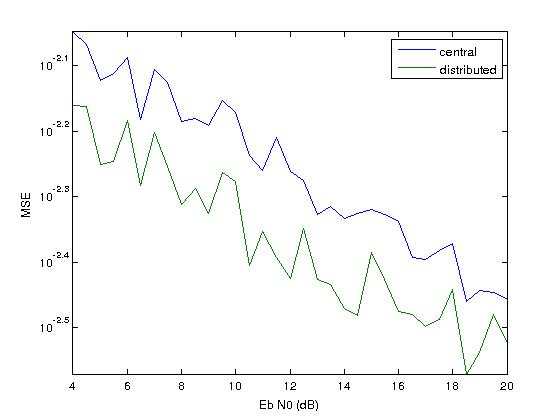
\includegraphics[height = 7.3 cm]{ebn0bbvsmse10ppnoH1logs.jpg}
\caption{Mse vs SNR for the sensing model, with AWGN only, showing the performance of distributed and centralised solvers}
\label{msevssnr0}
\end{figure}

\begin{figure}[h]
\centering
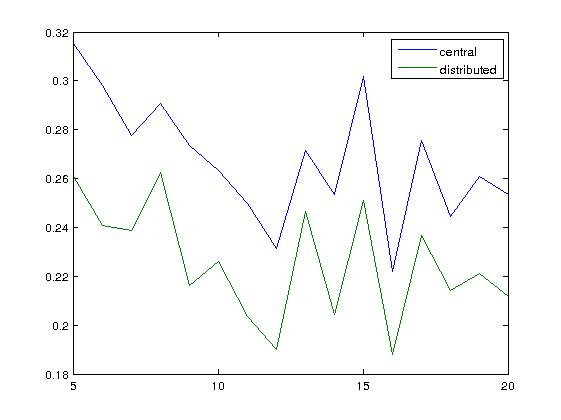
\includegraphics[height = 7.3 cm]{ebn0bbvsmse100ppwithH.jpg}
\caption{Mse vs SNR for the sensing model, showing the performance of distributed and centralised solvers}
\label{msevssnr1}
\end{figure}

\begin{figure}[h]
\centering
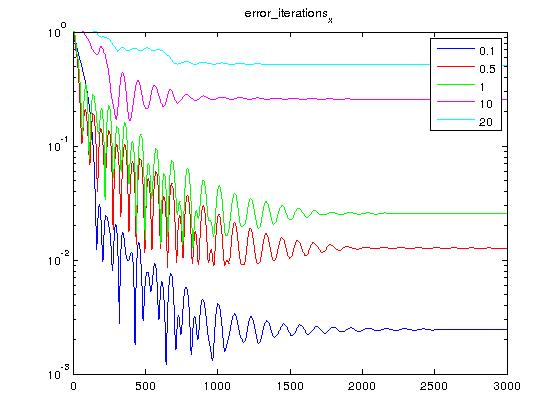
\includegraphics[height = 7.3 cm]{different_lambda.jpg}
\caption{The progress of the distributed solver as a function of the number of iterations, with different values of the regression parameter \(\lambda\)}
\label{fig:differentLambda}
\end{figure}

\begin{figure}[h]
\centering
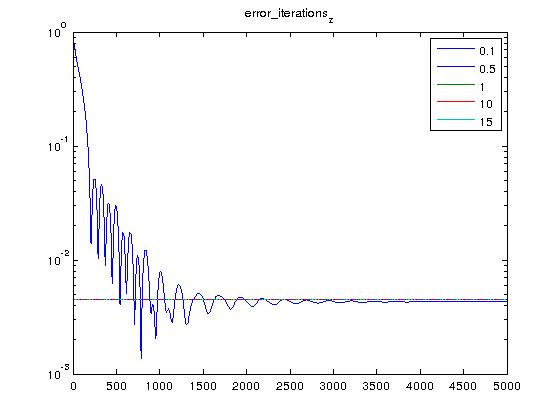
\includegraphics[height = 7.3 cm]{mse_iterations.jpg}
\caption{The progress of a distributed (blue) and a centralised (green) solver as a function of the number of iterations. The value of \(\lambda = 0.1\)}
\label{fig:erroriterations}
\end{figure}

\begin{figure}[h]
\centering
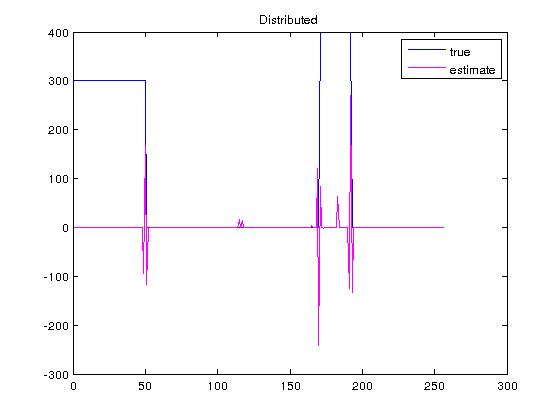
\includegraphics[height = 7.3 cm]{recon_spline.jpg}
\caption{The progress of a distributed (blue) and a centralised (green) solver as a function of the number of iterations. The value of \(\lambda = 0.1\)}
\label{fig:spline_recon}
\end{figure}

\begin{figure}[h]
\centering
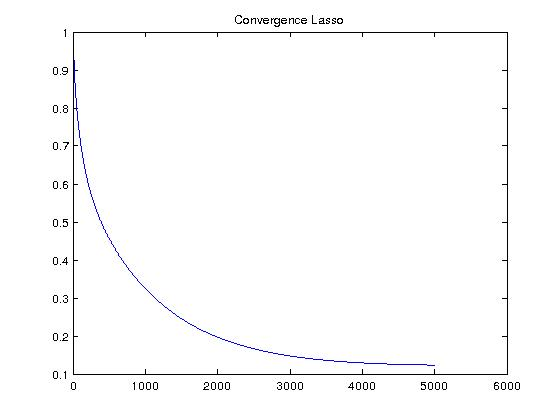
\includegraphics[height = 7.3 cm]{steps.jpg}
\caption{The progress of a distributed (blue) and a centralised (green) solver as a function of the number of iterations. The value of \(\lambda = 0.1\)}
\label{fig:steps_wavelets}
\end{figure}

\begin{figure}[h]
\centering
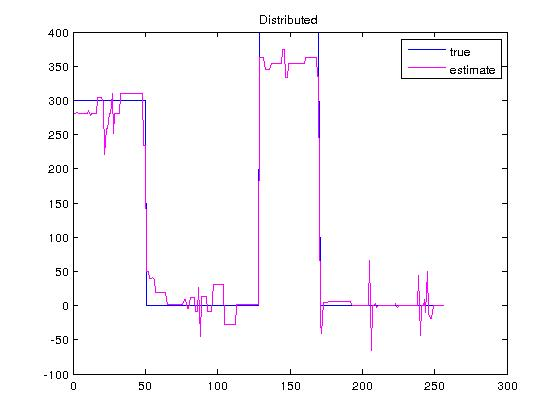
\includegraphics[height = 7.3 cm]{recon170815.jpg}
\caption{The progress of a distributed (blue) and a centralised (green) solver as a function of the number of iterations. The value of \(\lambda = 0.1\)}
\label{fig:wavelet_recon}
\end{figure}

\begin{figure}[h]
\centering
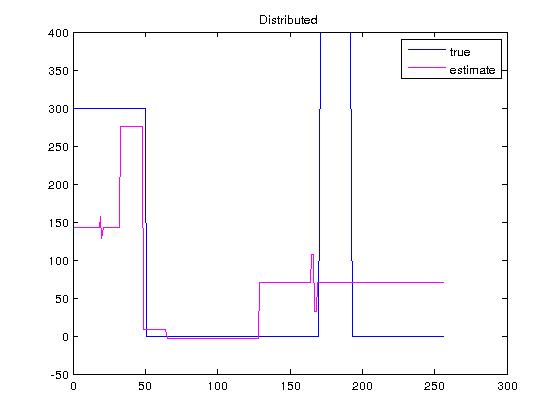
\includegraphics[height = 7.3 cm]{recon_new_bar.jpg}
\caption{The progress of a distributed (blue) and a centralised (green) solver as a function of the number of iterations. The value of \(\lambda = 0.1\)}
\label{fig:wavelet_recon_no_pwer_2}
\end{figure}

\begin{figure}[h]
\centering
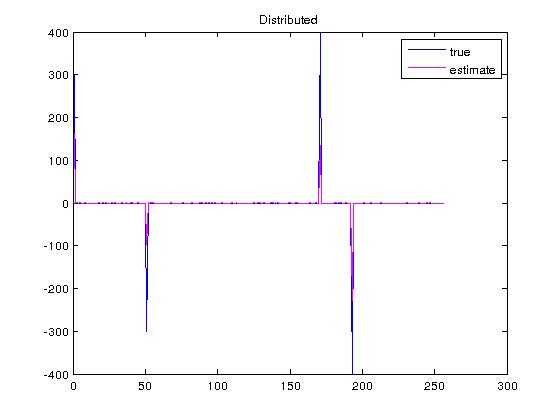
\includegraphics[height = 7.3 cm]{recon_difference.jpg}
\caption{The progress of a distributed (blue) and a centralised (green) solver as a function of the number of iterations. The value of \(\lambda = 0.1\)}
\label{fig:erroriterations}
\end{figure}

\begin{figure}[h]
\centering
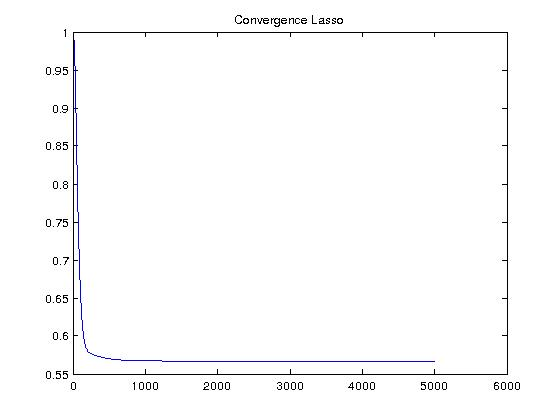
\includegraphics[height = 7.3 cm]{steps_difference.jpg}
\caption{The progress of a distributed (blue) and a centralised (green) solver as a function of the number of iterations. The value of \(\lambda = 0.1\)}
\label{fig:steps_difference}
\end{figure}

\begin{figure}[h]
\centering
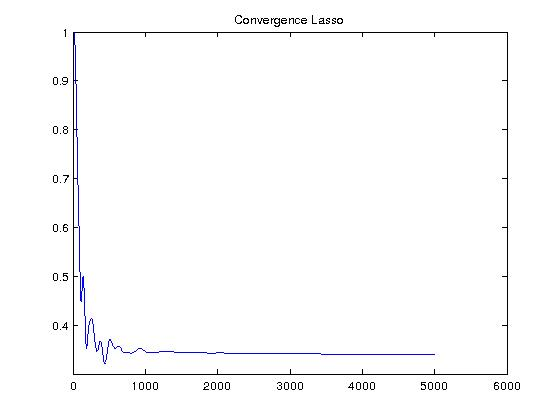
\includegraphics[height = 7.3 cm]{steps_splines.jpg}
\caption{The progress of a distributed (blue) and a centralised (green) solver as a function of the number of iterations. The value of \(\lambda = 0.1\)}
\label{fig:steps_splines}
\end{figure}

\begin{figure}[h]
\centering
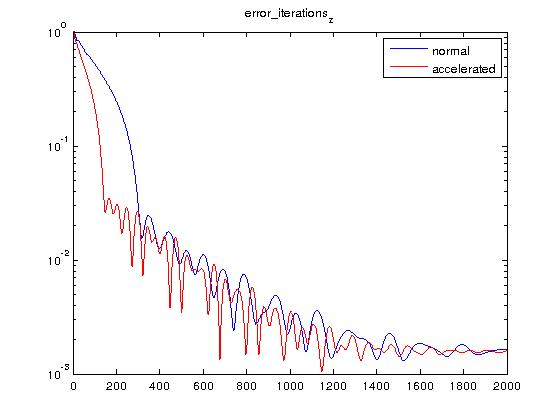
\includegraphics[height = 7.3 cm]{normalvsaccel.jpg}
\caption{The progress of a distributed (blue) and a centralised (green) solver as a function of the number of iterations. The value of \(\lambda = 0.1\)}
\label{fig:steps_splines}
\end{figure}

\section{Conclusions}
We have demonstrated an alternating direction algorithm for distributed optimisation with closed forms for the computation at each step, and discussed the statistical properties of the estimation. 

We have simulated the performance of this distributed algorithm for the distributed estimation of frequency spectra, in the presence of additive (white, Gaussian) and multiplicative (frequency flat) noise. We have shown that the algorithm is robust to a variety of SNRs and converges to the same solution as an equivalent centralised algorithm (in relative mean-squared-error).

We plan to work on larger, more detailed, models for the frequency spectra and to accelerate the convergence via Nesterov type methods to smooth the convergence of the distributed algorithm \cite{goldstein2014fast}. Specifically, we seek to dampen the ringing seen in Figure \ref{fig:erroriterations}
 
\chapter{Rectangular basis}

\section{Preliminaries}
Consider the basis defined by the function:

\begin{equation}
f_i\left(x\right) =
\begin{cases}
1 & \text{if } x \leq i \\
0 & \text{ otherwise } 
\end{cases}
\label{basis}
\end{equation}

That is, \(f_i\) is a left-hand step function. We define the inner product between two vectors as follows:

\begin{definition}
\begin{equation}
\langle x, y \rangle = x^T y = \sum_i x_i y_i
\end{equation}	
where \(x_i, y_i\) are the components of the vectors \(x,y\) in the \(i^{th}\) direction with respect to some basis vectors \(e_i\).
\end{definition}

We can define a matrix representation for the set of basis vectors \(f_i\), by taking all inner products between all pairs basis vectors:

\begin{definition}
\begin{equation}
F_{n, ij} = \langle f_i, f_j \rangle
\end{equation}

This matrix has the representation:

\begin{equation}
F_{ij} = min(i,j)
\end{equation}

An example of such a matrix is:

\begin{equation}
F_n= \begin{pmatrix}
 1 & 1 & 1 & 1  & 1 \\
  1 & 2 & 2 & 2  & 2\\
     1 & 2 & 3 & 3  & 3  \\
    1 & 2 & 3 & 4  & 4  \\
     1 & 2 & 3 & 4  & 5 
\end{pmatrix}
\end{equation}
\end{definition}

This matrix is invertible.

\begin{theorem}
\begin{equation}
det(F_n) = 1
\end{equation}
\end{theorem}
\begin{proof}
Consider the matrix \(F^n\). Subtract the \(n-1\)th column from the \(n\)th. We obtain a matrix with \(0\) on the final column except the entry \(F^n_(n,n) = 1\). Since the top \((n-1) \times (n-1)\) is \(F^{n-1}\) we find that 

\begin{equation}
det(F_n) = 1 \times det(F_{n-1})
\end{equation} 

By recursion and \(det(F_1) = 1\) we have \(det(F_n) = 1\).

\end{proof}

This matrix can be factorised as \(F = LL^T\) where 

\begin{equation}
L = \begin{pmatrix}
 1 & 0 & 0 & 0  & 0 \ldots 0 \\
  1 & 1 & 0 & 0  & 0 \ldots 0\\
     1 & 1 & 1 & 0  & 0 \ldots0  \\
    \ldots  \\
     1 & 1 & 1 & 1  & 1 \ldots 1 
\end{pmatrix}
\end{equation}

From this it follows that

\begin{equation}
F^{-1} = \begin{pmatrix}
 2 & -1 & 0 & 0  & 0 \ldots 0 \\
  -1 & 2 & -1 & 0  & 0 \ldots 0\\
     0 & -1 & 2 & -1  & 0 \ldots0  \\
    \ldots  \\
     0 & 0 & 0 & 0  \ldots -1 & 1 
\end{pmatrix}
\end{equation}

Another matrix we will use a lot of is:

\begin{equation}
D = \begin{pmatrix}
 1 & 0 & 0 & 0  & 0 \ldots 0 \\
  -1 & 1 & 0 & 0  & 0 \ldots 0\\
     0 & -1 & 0 & 0  & 0 \ldots0  \\
    \ldots  \\
     0 & 0 & 0 & 0  \ldots -1 & 1
\end{pmatrix}
\end{equation}

and by direct computation:

\begin{equation}
DL = I
\label{Dinv}
\end{equation}

\section{Spectrum Sensing}

We model our PSD signal \(g\) as a linear combination of the basis functions (\ref{basis}):

\begin{equation}
g\left(x\right) = \sum_i a_i f_i 
\label{basis-expansion}
\end{equation}

To find the \(a_i\), we correlate (take the inner product of) the signal against the basis (\ref{basis}).

\begin{definition}
\begin{align}
h_j &= \langle g, f_j \rangle \\
&= \sum_j g\left(x\right) f_j\left(x\right) \\
&= \sum_j a_i f_i\left(x\right) f_j\left(x\right) \\
&= a_i \langle f_i, f_j\rangle \\
&\left(= \sum_{x=1}^j g\left(x\right)\right)
\end{align}

In matrix language \(h = F a^T\). This is the inner product between the signal \(g\) and the basis functions \(f_i\).
\end{definition}

\begin{definition}
\begin{equation}
d_i\left(x\right) =
\begin{cases}
1 & \text{if } x = i \\
-1 & \text{if } x = i-1 \\
0 & \text{otherwise} 
\end{cases}
\end{equation}
i.e. \(d_i\) is the \(i^{th}\) row of the matrix \(D\).
\end{definition}

\begin{theorem}
\begin{equation}
D^Tg = a
\end{equation}
\end{theorem}
\begin{proof}
From the definition of \(g\) (\ref{basis-expansion})

\begin{align}
D^Tg &= D^T \sum_i a_i f_i \\
&= \sum_i a_i d_j^T f_i \\
&= a \langle d_j, f_i\rangle \\
&= a
\end{align}
as
\begin{equation}
\langle d_j, f_i \rangle = =
\begin{cases}
1 & \text{if } i \leq j \\
0 & \text{otherwise} 
\end{cases}
\end{equation}
\end{proof}

This means 

\begin{equation}
g = \left(D^T\right)^{-1} a =\left(D^{-1}\right)^T a
\end{equation}

so using (\ref{Dinv}), 

\begin{equation}
g = L^T a
\end{equation}

To recover \(\hat{a}\), we minimise

\begin{equation}
\vectornorm{h - Fa}_2^2
\end{equation}

in the noiseless case, and

\begin{equation}
\vectornorm{h_\varepsilon - Fa}_2^2 + \lambda\vectornorm{a}_1
\label{recon}
\end{equation}

in the noisy case, where 

\begin{equation}
\left(h_\varepsilon\right)_j = \langle\left(g+\varepsilon\right), f_j\rangle
\end{equation}

and \(\varepsilon \sim \mathcal{N}(0,\sigma^2\ I)\).

From \(\hat{a}\) we can recover \(\hat{g}\) from the following relation:

\begin{equation}
\hat{g} = L^{T} \hat{a}
\end{equation}


\section{Results}

\begin{figure}[h]
\centering
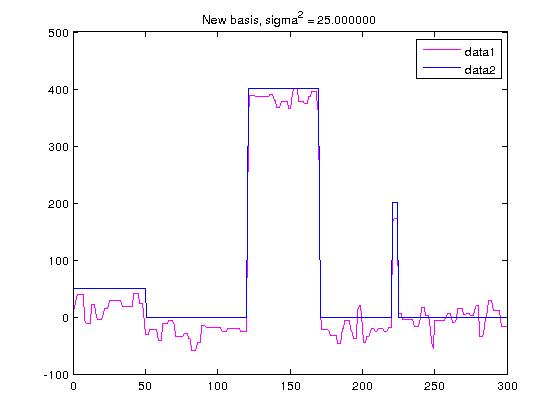
\includegraphics[height = 7.3 cm]{new_basis_25.jpg}
\caption{}
\label{fig:new_basis_25}
\end{figure}

\begin{figure}[h]
\centering
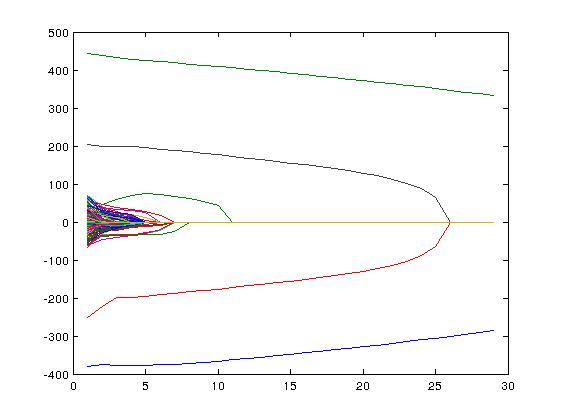
\includegraphics[height = 7.3 cm]{new_basis_different_lambdas.jpg}
\caption{}
\label{fig:new_basis_25}
\end{figure}

\begin{figure}[h]
\centering
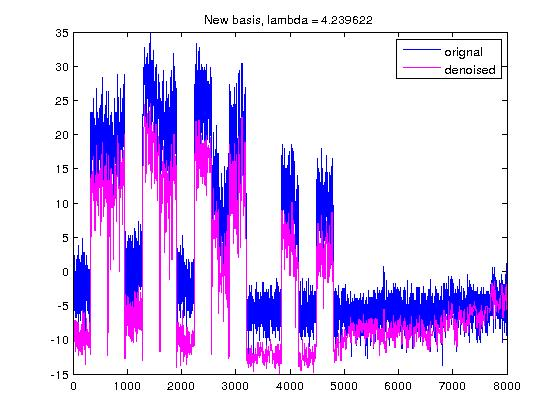
\includegraphics[height = 7.3 cm]{new_basis_ofcom_1.jpg}
\caption{}
\label{fig:new_basis_25}
\end{figure}
\begin{figure}[h]
\centering
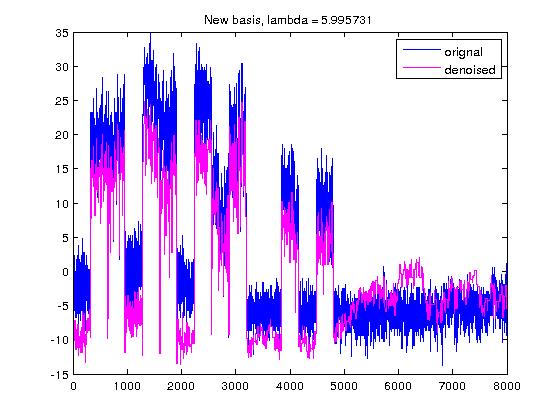
\includegraphics[height = 7.3 cm]{new_basis_ofcom_2.jpg}
\caption{}
\label{fig:new_basis_25}
\end{figure}
\begin{figure}[h]
\centering
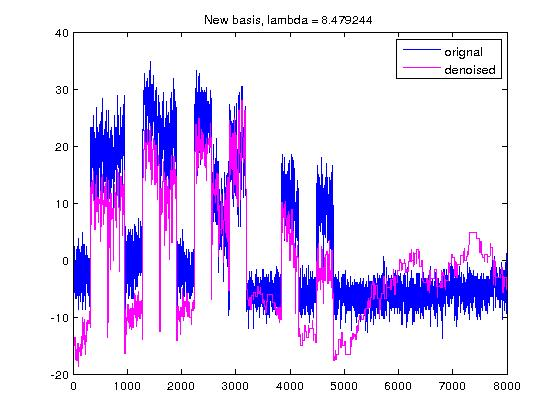
\includegraphics[height = 7.3 cm]{new_basis_ofcom_3.jpg}
\caption{}
\label{fig:new_basis_25}
\end{figure}
\begin{figure}[h]
\centering
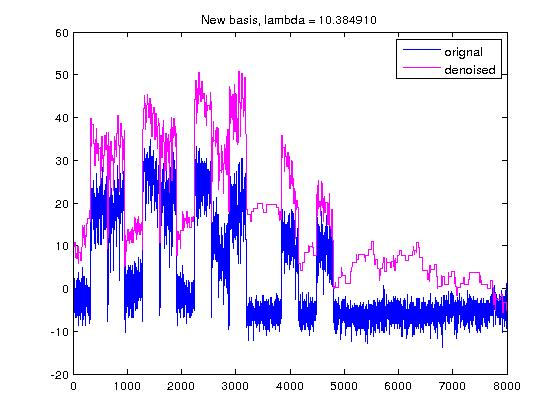
\includegraphics[height = 7.3 cm]{new_basis_ofcom_4.jpg}
\caption{}
\label{fig:new_basis_25}
\end{figure}

\begin{figure}[h]
\centering
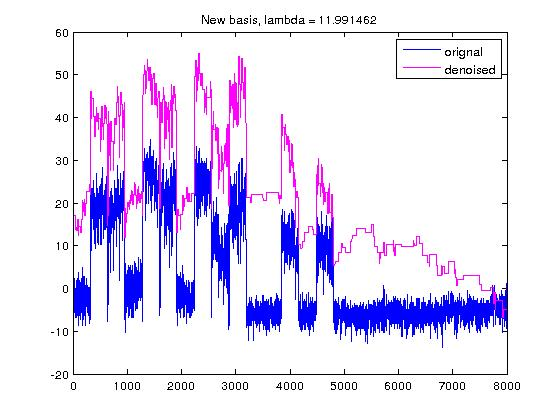
\includegraphics[height = 7.3 cm]{new_basis_ofcom_5.jpg}
\caption{}
\label{fig:new_basis_25}
\end{figure}
 

%----------------------------------------------------------------------------------------
%	THESIS CONTENT - APPENDICES
%----------------------------------------------------------------------------------------

\appendix % Cue to tell LaTeX that the following "chapters" are Appendices

% Include the appendices of the thesis as separate files from the Appendices folder
% Uncomment the lines as you write the Appendices

% Appendix A

\chapter{Appendix Title Here} % Main appendix title

\label{AppendixA} % For referencing this appendix elsewhere, use \ref{AppendixA}

Write your Appendix content here.
%\input{Appendices/AppendixB}
%\input{Appendices/AppendixC}

%----------------------------------------------------------------------------------------
%	BIBLIOGRAPHY
%----------------------------------------------------------------------------------------

%\printbibliography[heading=bibintoc]

%----------------------------------------------------------------------------------------

\end{document}